\section{System/Product design} \label{sec:design}
This section dives into the tracker's design, starting with establishing product requirements using an actor-oriented approach and addressing the \ac{PCB} design and case design for optimal functionality and user experience.
In between this, the implementation of software features and strategies for power minimisation to enhance battery life will be explored

\subsection{Development of product requirements}
\textit{The following section is a rough draft}
There are many different ways to go about product development and many different ways to get a design assignment. You can be assigned to design a product where the goals have been clearly defined in advance by others, you can be tasked with redesigning an already existing product with all of its inherent product requirements, you can get tasked to design a product for a client who most likely has thoughts, ideas and wants for that, or in our case, have a broad idea that you are trying to turn into a product.

One way to start developing product requirements for such a task is to think about use cases to look into competitors on the market, and compare their features, to get an idea if there is an opening in the market, and if not which requirements your product should have, to be able to compete against similar products.

On the market today, there are two major technologies for tracking objects: \ac{GPS} trackers and Bluetooth trackers.
\ac{GPS} trackers work individually and utilise the \ac{GNSS} network to track the position of the object, and then use \ac{GSM} or an \ac{LPWAN} like \ac{LoRaWAN} or Sigfox to broadcast the location.
Bluetooth trackers on the other hand connect to your or nearby phones and then use the phone's location and data connection, to broadcast its location.


% STORK: https://tektelic.com/wp-content/uploads/STORK-Asset-Tracker.pdf

The most popular Bluetooth trackers are the Apple AirTag\footnote{\url{https://www.apple.com/airtag/}} and Tile.
Pros:
\begin{itemize}
  \item Compact and Lightweight: Most Bluetooth trackers are small and lightweight, making them easy to attach to various items without adding bulk or weight.
  \item Affordable: Bluetooth trackers are generally more affordable than \ac{GPS} trackers, making them accessible to many users.
  \item Long Battery Life: Many Bluetooth trackers come with replaceable batteries that last several months or even years, ensuring prolonged usability without frequent recharging.
  \item Can use \ac{UWB} for really precise close-by tracking.
\end{itemize}

Cons:
\begin{itemize}
  \item Limited Range: Bluetooth trackers have a limited range compared to \ac{GPS} trackers, typically around 100-200 feet indoors and up to 300 feet outdoors, which may restrict their effectiveness in certain situations.
  \item Dependency on Smartphone: Bluetooth trackers rely on the connection to a smartphone or tablet via Bluetooth, so if the smartphone's battery dies or Bluetooth is turned off, tracking functionality may be compromised.
  \item Lack of \ac{GPS}: Unlike \ac{GPS} trackers, Bluetooth trackers do not provide real-time location updates or tracking over long distances, limiting their usefulness for locating items beyond the Bluetooth range.
  \item Vendor-specific: Bluetooth trackers are often designed to work exclusively with devices from a specific manufacturer or ecosystem. For example, Apple's AirTag is optimised for iPhone use and relies on the Find My app, while other Bluetooth trackers may be tailored for Android devices or specific third-party platforms. This vendor specificity limits cross-platform compatibility and may exclude users who do not use compatible devices, reducing the overall accessibility and interoperability of Bluetooth trackers.
\end{itemize}

Pros and cons of \ac{GPS} trackers:\\
Pros:
\begin{itemize}
  \item Accurate Tracking: \ac{GPS} trackers provide real-time and precise location data, allowing users to monitor the exact whereabouts of their belongings or vehicles.
  \item Long-Distance Coverage: \ac{GPS} trackers can track items over long distances, making them suitable for locating assets that may travel far from their original location.
  \item Wide Compatibility: \ac{GPS} trackers are generally compatible with various devices and platforms, offering broader accessibility to users regardless of their preferred devices or ecosystems.
  \item Geofencing Capabilities: Many \ac{GPS} trackers offer geofencing features, enabling users to set virtual boundaries and receive alerts when their tracked items enter or exit designated areas.
\end{itemize}

Cons:
\begin{itemize}
  \item Subscription Fees: Some \ac{GPS} trackers require subscription plans for accessing features like real-time tracking or historical data, adding ongoing costs for users beyond the initial purchase price.
  \item Power Consumption: \ac{GPS} trackers often consume more power than Bluetooth trackers, leading to shorter battery life or the need for frequent recharging.
  \item Reliance on Satellite Signals: \ac{GPS} trackers rely on satellite signals for location tracking, which may be obstructed or limited in certain environments such as indoors or urban areas with tall buildings, reducing tracking accuracy or effectiveness.
  \item Higher Cost: \ac{GPS} trackers tend to be more expensive than Bluetooth trackers due to their advanced features and capabilities, potentially making them less accessible to budget-conscious users.
\end{itemize}

\begin{table}[H]
\scriptsize
\caption{Other tracker}
\label{tab:other_tracker}
\begin{tabular}{llllllp{3cm}}
 & Price & Size [mm] & Battery & Mont. cost & Track. dist. & Features \\
\hline
Apple AirTag & 300 & $32 \times 32 \times 8$ & Up to 1 yr & Free & \SI{30}{\meter} & \ac{BLE}, speaker, many\newline people own iPhones \\
\makecell[l]{Tile mate\\\,} & \makecell[l]{>260\\\,} & \makecell[l]{$38 \times 38 \times 7$\\\,} & \makecell[l]{Up to 1 yr\\\,} & \makecell[l]{Free\\\,} & \makecell[l]{\SI{76}{\meter}\\\,} & Watertight (IP67), different forms, speaker \\
\makecell[l]{MiniFinder Pico\\\,} & \makecell[l]{2950\\\,} & \makecell[l]{$61 \times 41 \times 16$\\\,} & \makecell[l]{40 h (5 min interv.),\\20 days (standby)} &  &  &  \\
\makecell[l]{MiniFinder nano\\\,} & \makecell[l]{3000\\\,} & \makecell[l]{$47 \times 41 \times 16$\\\,} & \makecell[l]{36 h active,\\ 120 h stand-by} &  &  &  \\
Minifinder Extreme & 3600 & \makecell[l]{$88 \times 62 \times 34$\\} & 10 yr (standby) &  &  &  \\
Cobblestone Pro & 1500 & \makecell[l]{$64 \times 64 \times 23$\\} & 4 yr (1 update/day) & Free &  &  \\
Zmartgear Sigfox & 1300 & \makecell[l]{$42 \times 24 \times 17$\\} & 3 months (standby) & 3 yr free &  &  \\
Odin tracker & 2500 & \makecell[l]{$58 \times 41 \times 19$\\} & 10 yr (3000 tracks) & 0 &  &  \\
\end{tabular}
\end{table}

\iffalse
\textbf{Popular trackers:}\\
\textbf{Apple AirTag} (\ac{BLE})
\begin{itemize}[label={}, noitemsep, leftmargin=0pt]
    \item Price: \SI{300}{\dkk}
    \item Size: \si{31,9} × \si{31,9} × \SI{8}{\milli\meter}
    \item Battery life: Up to 1 year
    \item Monthly cost: Free
    \item Tracking distance: \SI{30}{\meter}
    \item Other notable features: \ac{UWB}, speaker, many people own iPhones
\end{itemize}

\textbf{Tile mate} (Bluetooth)
\begin{itemize}[label={}, noitemsep, leftmargin=0pt]
    \item Price: from \SI{260}{\dkk}
    \item Size: \si{37,8} × \si{37,8} × \SI{7.2}{\milli\meter}
    \item Battery life: Up to 1 year
    \item Monthly cost: Free
    \item Tracking distance: \SI{76}{\meter}
    \item Other notable features: speaker, can be bought in different forms, watertight (IP67)
\end{itemize}

\textbf{MiniFinder Pico} (\ac{GPS})
\begin{itemize}[label={}, noitemsep, leftmargin=0pt]
    \item Price: \SI{2950}{\dkk}
    \item Size: \si{61} × \si{41} × \SI{16}{\milli\meter}
    \item Battery life: \si{36}-\SI{40}{\hour} with \SI{5}{\minute} intervals, 20 days on standby
    \item Weight: \SI{40}{\gram}
    \item Network: 4G
    \item Monthly cost: \SI{159}{\dkk} + \SI{65}{\dkk} for non EU-countries
    \item \ac{GPS} start-on time: Active \SI{1}{\second}, Hot \SI{5}{\second}, Cold \SI{15}{\second}
    \item Other notable features: waterproof, g-sensor, panic button
\end{itemize}

\textbf{MiniFinder nano} (\ac{GPS} + \ac{BLE} + Wi-Fi)
\begin{itemize}[label={}, noitemsep, leftmargin=0pt]
    \item Price: \SI{3000}{\dkk}
    \item Size: \si{47} × \si{41} × \SI{16}{\milli\meter}
    \item Battery life: \SI{36}{\hour} active use, \SI{120}{\hour} hours stand-by use
    \item Monthly cost: \SI{159}{\dkk} + \SI{65}{\dkk} for non EU-countries
    \item Weight: \SI{60}{\gram}
    \item Network: 4G
    \item \ac{GPS} start-on time: Active \SI{1}{\second}, Hot \SI{5}{\second}, Cold \SI{15}{\second}
    \item Other notable features: watch format, call function and panic button, fall alarm
\end{itemize}

\textbf{Minifinder Extreme} (\ac{GPS})
\begin{itemize}[label={}, noitemsep, leftmargin=0pt]
    \item Price: \SI{3600}{\dkk}
    \item Size: \si{88} × \si{62} × \SI{34}{\milli\meter}
    \item Battery life: 10 years on standby
    \item Weight: \SI{290}{\gram}
    \item Network: 4G
    \item \ac{GPS} start-on time: Active \SI{1}{\second}, Hot \SI{35}{\second}, Cold \SI{45}{\second}
    \item Monthly cost: \SI{159}{\dkk} + \SI{65}{\dkk} for non EU-countries
    \item Other notable features: magnet montage
\end{itemize}

\textbf{Cobblestone Pro} (\ac{GPS})
\begin{itemize}[label={}, noitemsep, leftmargin=0pt]
    \item Price: \SI{1500}{\dkk}
    \item Size: \si{64} × \si{64} × \SI{23}{\milli\meter}
    \item Network: 4G
    \item Weight: \SI{100}{\gram}
    \item Battery life: \SI{4}{\year} (1 position update/day)
    \item Yearly cost: Free (\SI{400}{\dkk} for battery change \& for coverage upgrade)
    \item Other notable features: shockproof
\end{itemize}

\textbf{Zmartgear Sigfox tracker}
\begin{itemize}[label={}, noitemsep, leftmargin=0pt]
    \item Price: \SI{1300}{\dkk}
    \item Size: \si{42} × \si{24} × \SI{17}{\milli\meter}
    \item Weight: \SI{15}{\gram}.
    \item Battery life: 3 months on standby
    \item Yearly cost: \SI{3}{\year} free
    \item Network: Sigfox.
    \item Other notable features: cheaper than GSM, only updates when the device has laid still for \SI{2}{\minute}
\end{itemize}

Odin tracker
\begin{itemize}[label={}, noitemsep, leftmargin=0pt]
    \item Price: \SI{2500}{\dkk}
    \item Size: \si{58} × \si{41} × \SI{19}{\milli\meter}
    \item Weight: \SI{40}{\gram}
    \item Network: 5G NB-IOT
    \item Battery life: up to 10 years (3000 tracks)
    \item Yearly cost: 0
    \item Other notable features: uses Li-SOCI2 2/3AA battery
\end{itemize}
\fi

\subsubsection{Use cases}
In this subsection, we will describe different use cases. We will examine this through desk research and brainstorming.

Vehicle Tracking: \ac{GPS} trackers can be installed in cars, trucks, or fleet vehicles to monitor their location, speed, and route in real time. This is useful for fleet management, theft prevention, and optimising logistics.

Asset Tracking: \ac{GPS} trackers can be attached to valuable assets such as equipment, machinery, or containers to monitor their location and movement. This helps businesses track inventory, prevent loss or theft, and improve asset utilisation.

Personal Safety: \ac{GPS} trackers can be carried by individuals, such as elderly people, children, or outdoor enthusiasts, to provide their location in emergencies. This allows caregivers or authorities to locate them quickly and provide assistance if needed.

Pet Tracking: \ac{GPS} trackers attached to pet collars enable owners to monitor their pet's location and receive alerts if they wander outside a designated area. This helps prevent lost pets and facilitates quick recovery if they go missing.

Wildlife and Environmental Monitoring: \ac{GPS} trackers can be attached to wildlife or environmental sensors to track the movement and behaviour of animals, monitor habitat use, and collect data on environmental conditions such as temperature, humidity, or pollution levels.

Package Delivery: \ac{GPS} trackers can be used by courier services and delivery companies to track the location of packages in transit, provide customers with real-time delivery updates, and ensure timely and accurate delivery.

Knowing the product specifications of similar products and potential use cases can help us develop our product requirements.
Another thing we can do, to make sure that our requirements turn into a product that has relevance in the world, is to ask potential uses within the found use cases. If we get their thoughts on board, there is a greater chance that we will end up with a product that people will buy.

\subsubsection{Design criteria}
%In this section, with an actor-oriented design approach, we will set up design requirements for the final product, against which we can measure it at the end of the report/project.
%These will be set up in requirements (need to have), criteria (measurable requirements that can be adjusted), and wishes (nice to have).

\textbf{Initial design requirements}
\begin{table}[H]
\centering
\caption{Product requirments}
\label{tab:product_requirements}
\begin{tabular}{lp{12cm}}
\textbf{Category} & \textbf{Requirement}                                                                                                \\
Design            & Should be smaller than 40x40x20mm                                                                                   \\
                  & Should preferably be built in a size, and with a method that allows for multiple applications, e.g., wearable \\
                  & Should be weather resistant                                                                                         \\
                  & Should have an on/off button                                                                                        \\
                  & Should use a standard replaceable battery                                                                          \\
                  & Should have a wake-up button                                                                                       \\
Technical details & Should have a battery life of minimum 10000 indoor tracings                                                        \\
                  & Should have a battery life of minimum 4000 outdoor tracings                                                        \\
                  & Should turn on within \SI{10}{\second} from standby                                                                      \\
                  & Should turn on within \SI{60}{\second} from cold boot                                                                    \\
                  & Should go to deep sleep when not moving                                                                             \\
                  & Should automatically determine whether to use W-Fi or \ac{GNSS}                                                          \\
                  & Should have an accuracy of $\pm$50 meter                                                                              
\end{tabular}%
\end{table}

Other requirements to consider:
Price
Number of components
Reliability
Repair-ability
Operating costs

\subsection{Hardware design decisions}
Building a geolocation tracker requires transmitters, receivers, and most importantly, a device which controls the whole system. Furthermore, efficient communication between the single elements is important and will be investigated in this project. The following sections describe and discuss these aspects, emphasising challenges and pitfalls.

\subsubsection{Microcontroller}
For the main communication of the tracker, the project uses an ultra-low-power Arm\textsuperscript{\textregistered} Cortex\textsuperscript{\textregistered}-M4 32-bit \hyperref[bom:stm32l476]{STM32L476} chip (datasheet: \sbref{app:hardware:stm32l476rg}). It has \SI{512}{\kilo\byte} flash and a built-in internal voltage regulator and voltage scaling, that makes the chip particularly suited for portable battery-supplied products, down to \SI{1.71}{\volt} \cite{STM32L4_application_note}. It also possesses \ac{SPI} and \ac{I2C} for communication with different chips on the \ac{PCB}, and \ac{USART} for debugging sent to the user's machine. As the size of the firmware is around \SI{250}{\kilo\byte}, the chip does not need more than \SI{512}{\kilo\byte} in flash memory.

\begin{figure}[H]
    \centering
    \begin{subfigure}{.45\textwidth}
      \centering
      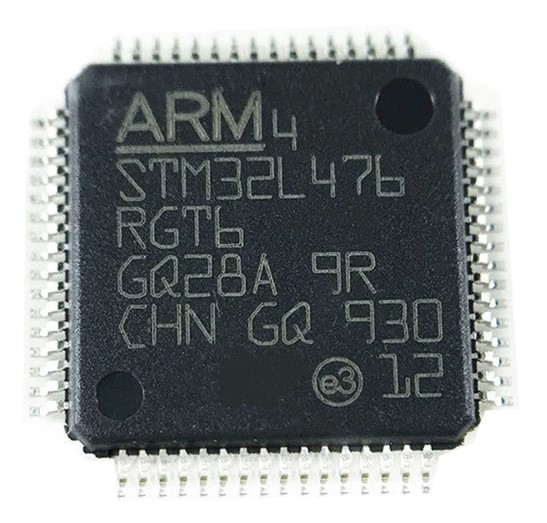
\includegraphics[width=0.7\textwidth]{figures/STM32L476.jpg}
    \end{subfigure}
    \begin{subfigure}{.45\textwidth}
      \centering
      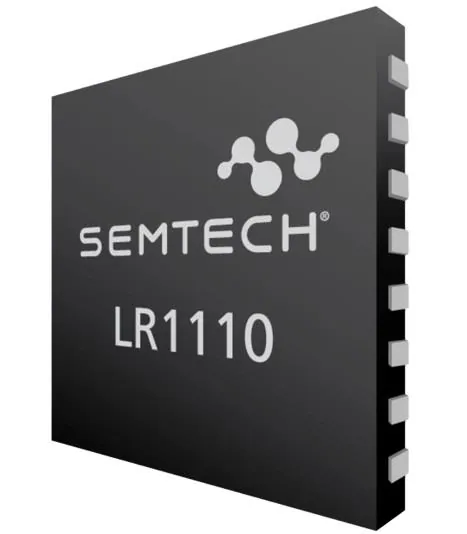
\includegraphics[width=0.55\textwidth]{figures/LR1110.png}
    \end{subfigure}
    \caption{STM32L476 (left) and LR1110 (right).}
    \label{fig:chips}
\end{figure}

\subsubsection{RF Transceiver and Receiver}
The \hyperref[bom:lr1110]{LR1110} chip (datasheet: \sbref{app:hardware:lr1110}) is a \ac{LoRa} RF Transceiver with inbuilt Wi-Fi and \ac{GNSS} scanner and is used for geolocation. Wi-Fi includes scanning for 802.11b/g/n Wi-Fi access point \ac{MAC} addresses (\SI{2.4}{\giga\hertz}), while the \ac{GNSS} scanning searches for \ac{GPS}\footnote{GPS: \url{https://www.gps.gov/}}, BeiDou\footnote{BeiDou Navigation Satellite System: \url{http://en.beidou.gov.cn/}}, and geostationary satellite signals. \ac{GNSS} and Wi-Fi scan data is collected on the device and sent to a cloud-based solver to resolve into a position. Semtech provides a Cloud API (fees apply).
cite to LR1110 driver \cite{lr11xx_driver}.

\subsubsection{Temperature Compensated Crystal Oscillator (TCXO)}
A \SI{32}{\mega\hertz} crystal oscillator is the cheapest and lowest power-consuming approach to provide the \SI{32}{\mega\hertz} clock reference to the LR1110 \cite[p.~50]{LR1110_user_manual}.
A \SI{32}{\mega\hertz} \ac{TCXO}\sbref{app:hardware:tcxo} and a \SI{32.768}{\kilo\hertz} clock source are mandatory by the LR1110 for any \ac{GNSS} operation. Further is the \ac{TCXO} a feature to minimise the power consumption required to perform outdoor geolocation \cite[p.~51, p.~132]{LR1110_user_manual}. The heat of the surroundings influences the crystal oscillators, so no copper planes have been added on the \ac{PCB} where crystal oscillators are placed. %Hvad gør forskellen på 1.6V eller 3.3V supply? 

\subsubsection{Accelerometer}
We are implementing an accelerometer to determine if the tracker has been still for a long time or has suddenly moved. We chose \hyperref[bom:lis2de12]{LIS2DE12} (datasheet: \sbref{app:hardware:lis2de12}), an ultra-low-power high-performance 3-axis femto accelerometer. \textit{Femto} meaning that it can detect accelerations on the order of femtometers per second squared (\SI{}{\femto\meter/\second^2}), which is a prefix denoting one quadrillionth ($10^{-15}$) and therefor incredibly small. It has \ac{SPI} and \ac{I2C}, but because \ac{I2C} uses much less power because of the slower speed, we will use that communication protocol - we don't need to send a lot of data back and forth fast. The wiring diagram of the accelerometer can be seen in fig.~\ref{fig:schematic:LIS2DE12} and as a simple block diagram in fig.~\ref{fig:schematic:accelerometer_halleffectsensor}.

\begin{figure}[H]
  \centering
  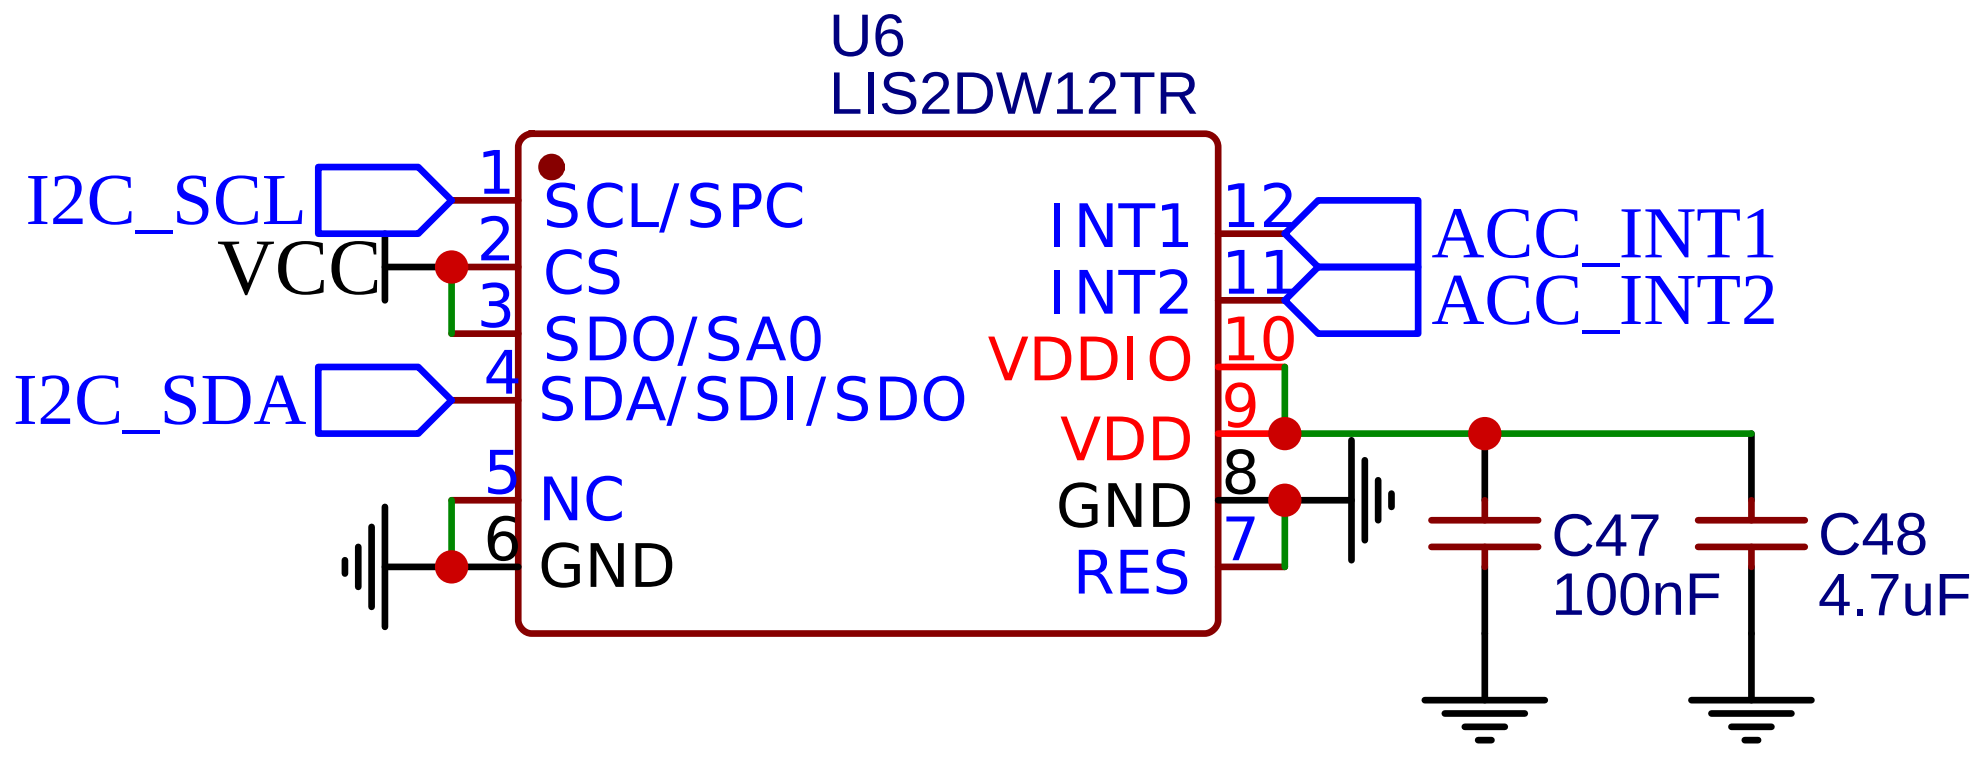
\includegraphics[width=0.6\textwidth]{figures/LIS2DE12.png}
  \caption{Wiring diagram of LIS2DE12.}
  \label{fig:schematic:LIS2DE12}
\end{figure}

\textit{C47} and \textit{C48} are defined from the datasheet \sbref{app:hardware:lis2de12}, p. 19). The accelerometer has two independent programmable interrupt generators for free-fall and motion detection. We will use both (\textit{ACC\_INT1} and \textit{ACC\_INT2}) to determine if the tracker has moved.

table 3.2.1 

Do we need to enable all axes?

It also has click-interrupt which could be used to wake up the tracker or configure it.

\begin{figure}[H]
    \centering
    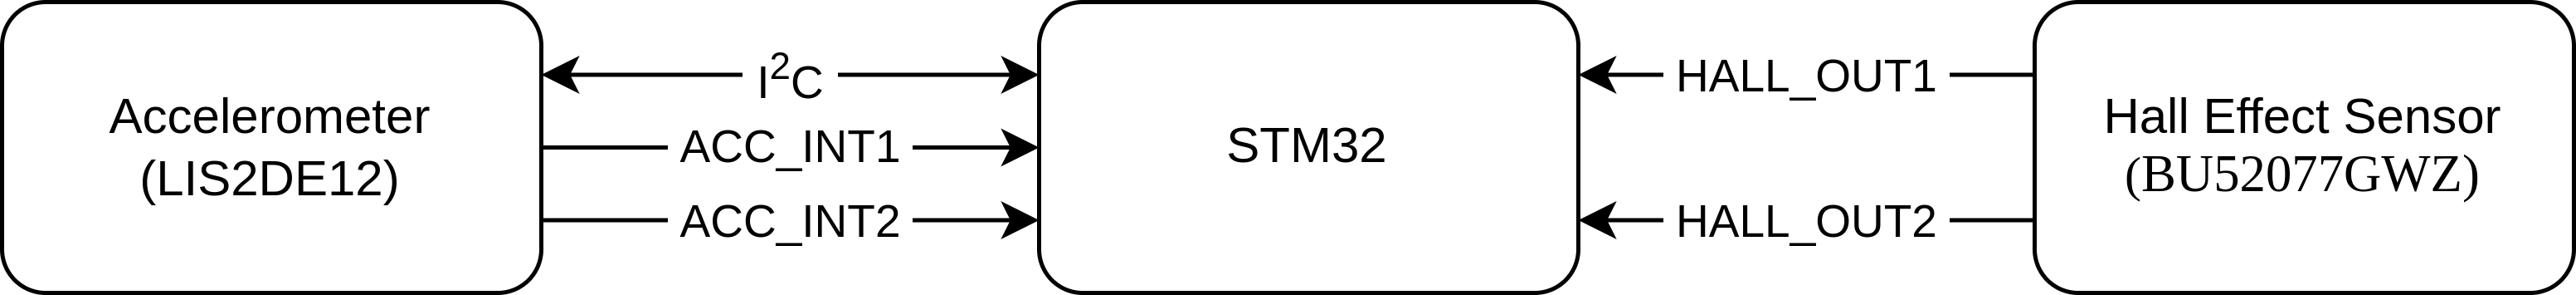
\includegraphics[width=0.9\textwidth]{figures/schematic_flow.png}
    \caption{Interface between STM32 and accelerometer and hall effect sensor.}
    \label{fig:schematic:accelerometer_halleffectsensor}
\end{figure}

\subsubsection{Hall Effect/Magnetic Sensors}
We are implementing a hall effect sensor to make the tracker waterproof and easier to turn on and off. We chose \hyperref[bom:bu52077gwz]{BU52077GWZ} (datasheet: \sbref{app:hardware:BU52077GWZ}) because it has a typical operational current of \SI{5}{\micro\ampere} and can operate at a voltage down to \SI{1.65}{\volt} which is suitable for this project. It has a normal \ac{GPIO} interface and is therefore easy to implement with a simple interrupt on the STM32. This hall effect chip is therefore ideal to work without application. The wiring diagram of the hall effect sensor can be seen in fig.~\ref{fig:schematic:BU52077GWZ} and as a simple block diagram in fig.~\ref{fig:schematic:accelerometer_halleffectsensor}.

\begin{figure}[H]
  \centering
  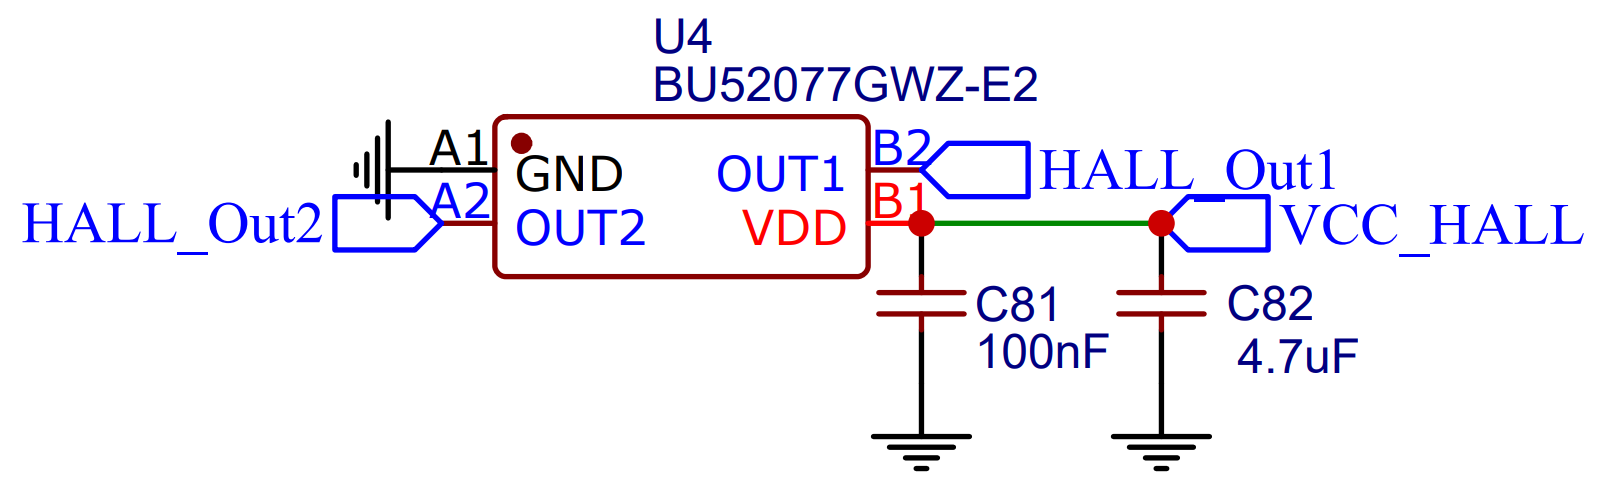
\includegraphics[width=0.6\textwidth]{figures/Hall.PNG}
  \caption{Wiring diagram of BU52077GWZ.}
  \label{fig:schematic:BU52077GWZ}
\end{figure}

\textit{HALL\_OUT1} is triggered when reacting to the south pole of a magnet, and \textit{HALL\_OUT2} is triggered when responding to the magnet's north pole. Therefore, the chip is ideal to switch to turn on and off the tracker.

\subsubsection{GNSS antenna}
Ceramic antenna
We are using a passive \ac{GNSS} antenna which means it has no external electrical components, as all the filtering and powering of the antenna is done directly on the \ac{PCB}.

\hyperref[bom:bga524n6e6327]{BGA 524N6 E6327} (datasheet: \sbref{app:hardware:bga524n6e6327})

\begin{figure}[H]
    \centering
    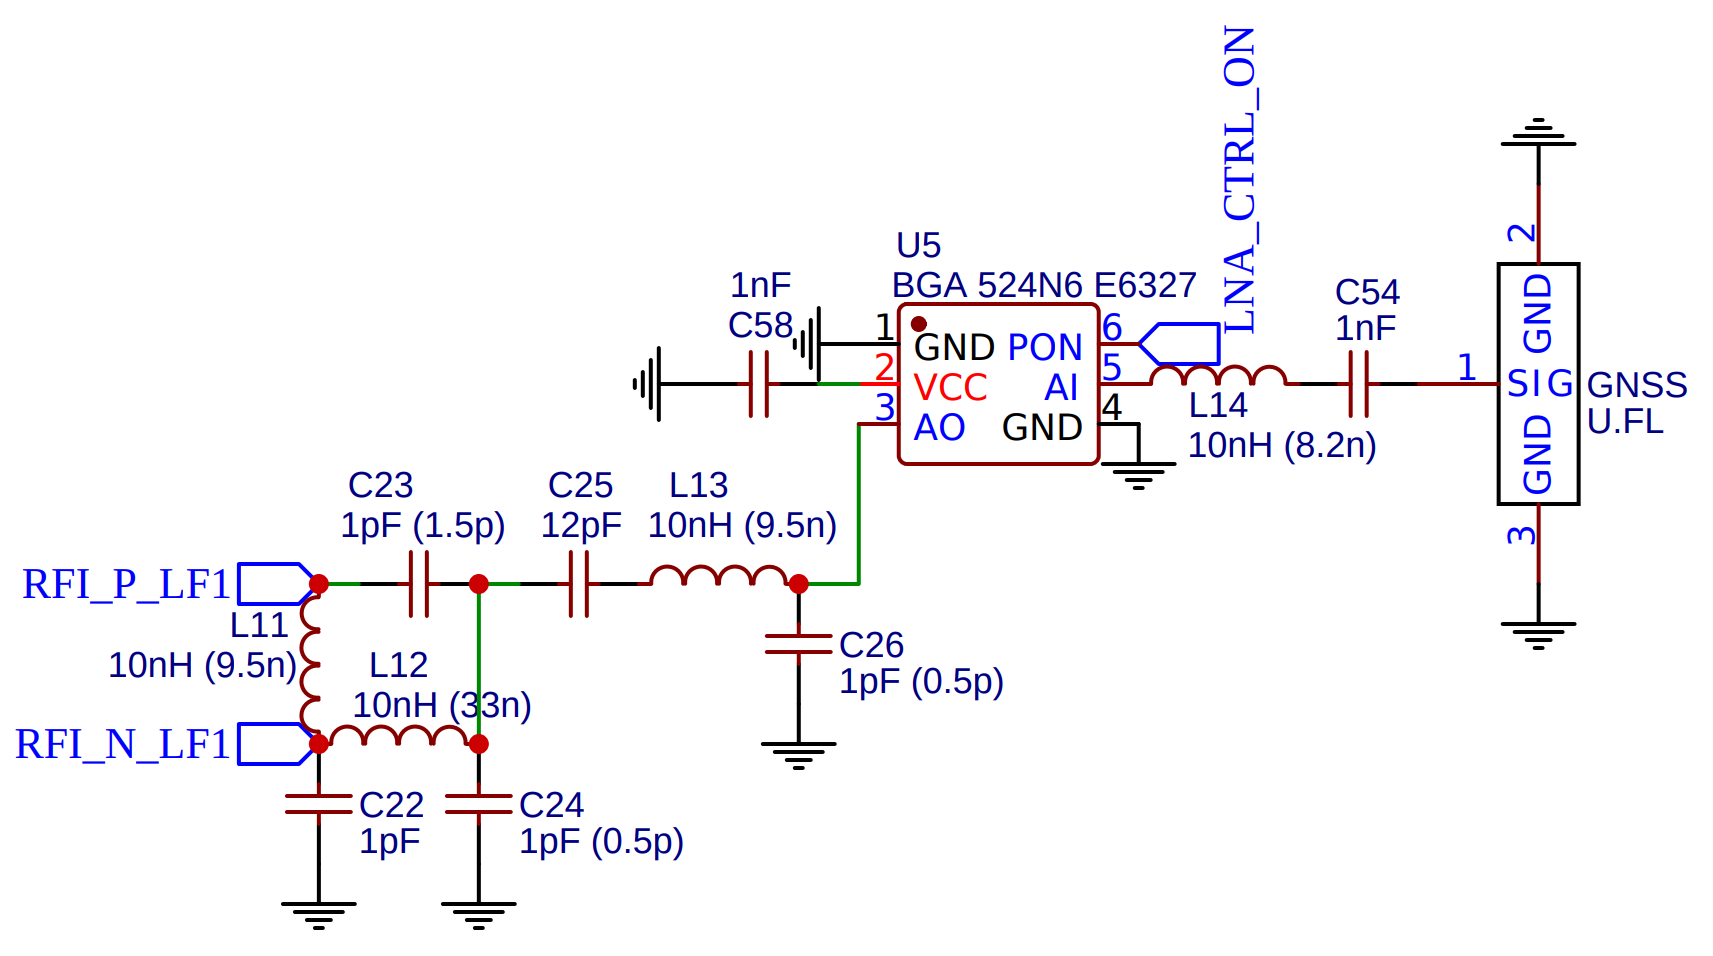
\includegraphics[width=0.9\textwidth]{figures/BGA524N6E6327.png}
    \caption{Wiring diagram of BGA 524N6 E6327.}
    \label{fig:schematic:bga524n6e6327}
\end{figure}

\subsection{Flash and debug a STM32 chip} \label{sec:flash_debug_stm32}
Flashing and debugging any STM32 chip is straightforward. All that is needed is an ST-LINK/V2-1\footnote{\url{https://www.st.com/en/development-tools/st-link-v2.html}} or any STM32 Nucleo board (which already has an ST-LINK/V2-1 built-in). The ST-LINK/V2-1 is connected to the STM32 chip through the \ac{SWD} interface, which is a two-wire interface consisting of a clock (\textit{SWDCLK}) and a data line (\textit{SWDIO}). 

\begin{figure}[H]
  \centering
  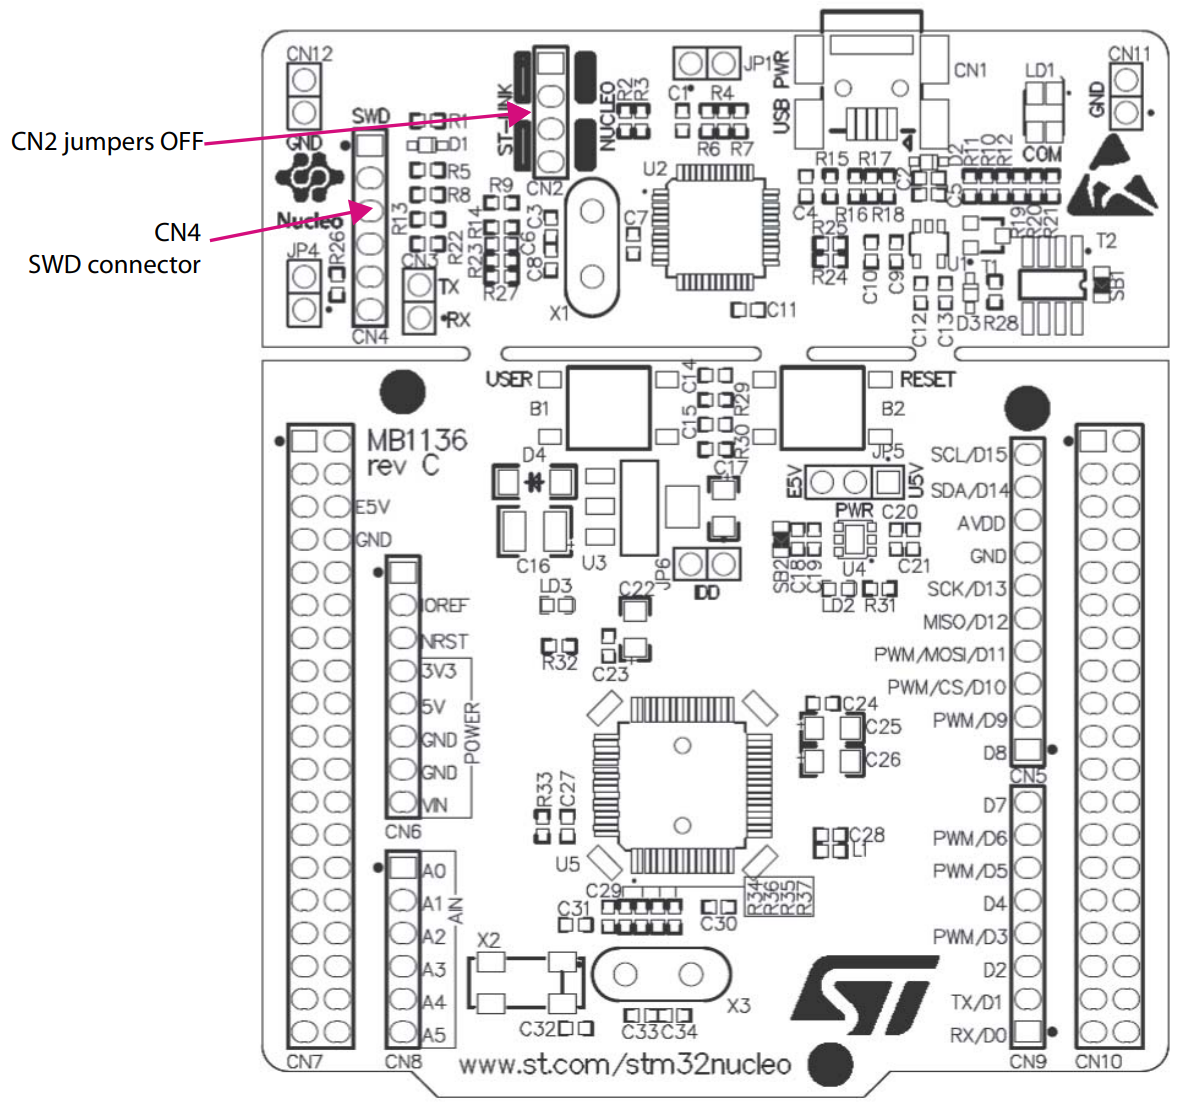
\includegraphics[width=0.7\textwidth]{figures/Nucleo_SWD.png}
  \caption{Using ST-LINK/V2-1 to program the STM32 chip on an external application \cite[p.~19]{STM32_Nucleo_user_manual}.}
  \label{fig:nucleo_swd}
\end{figure}

Per default, the ST-LINK/V2-1 is connected to the in-built STM32-chip on the STM32 Nucleo board. For flashing and debugging the STM32-chip on an external application remove the two jumpers from \textit{CN2} as illustrated in fig.~\ref{fig:nucleo_swd}, and connect the application to the \textit{CN4} debug connector according to fig.~\ref{fig:schematic_stlink}.

\begin{figure}[H]
  \centering
  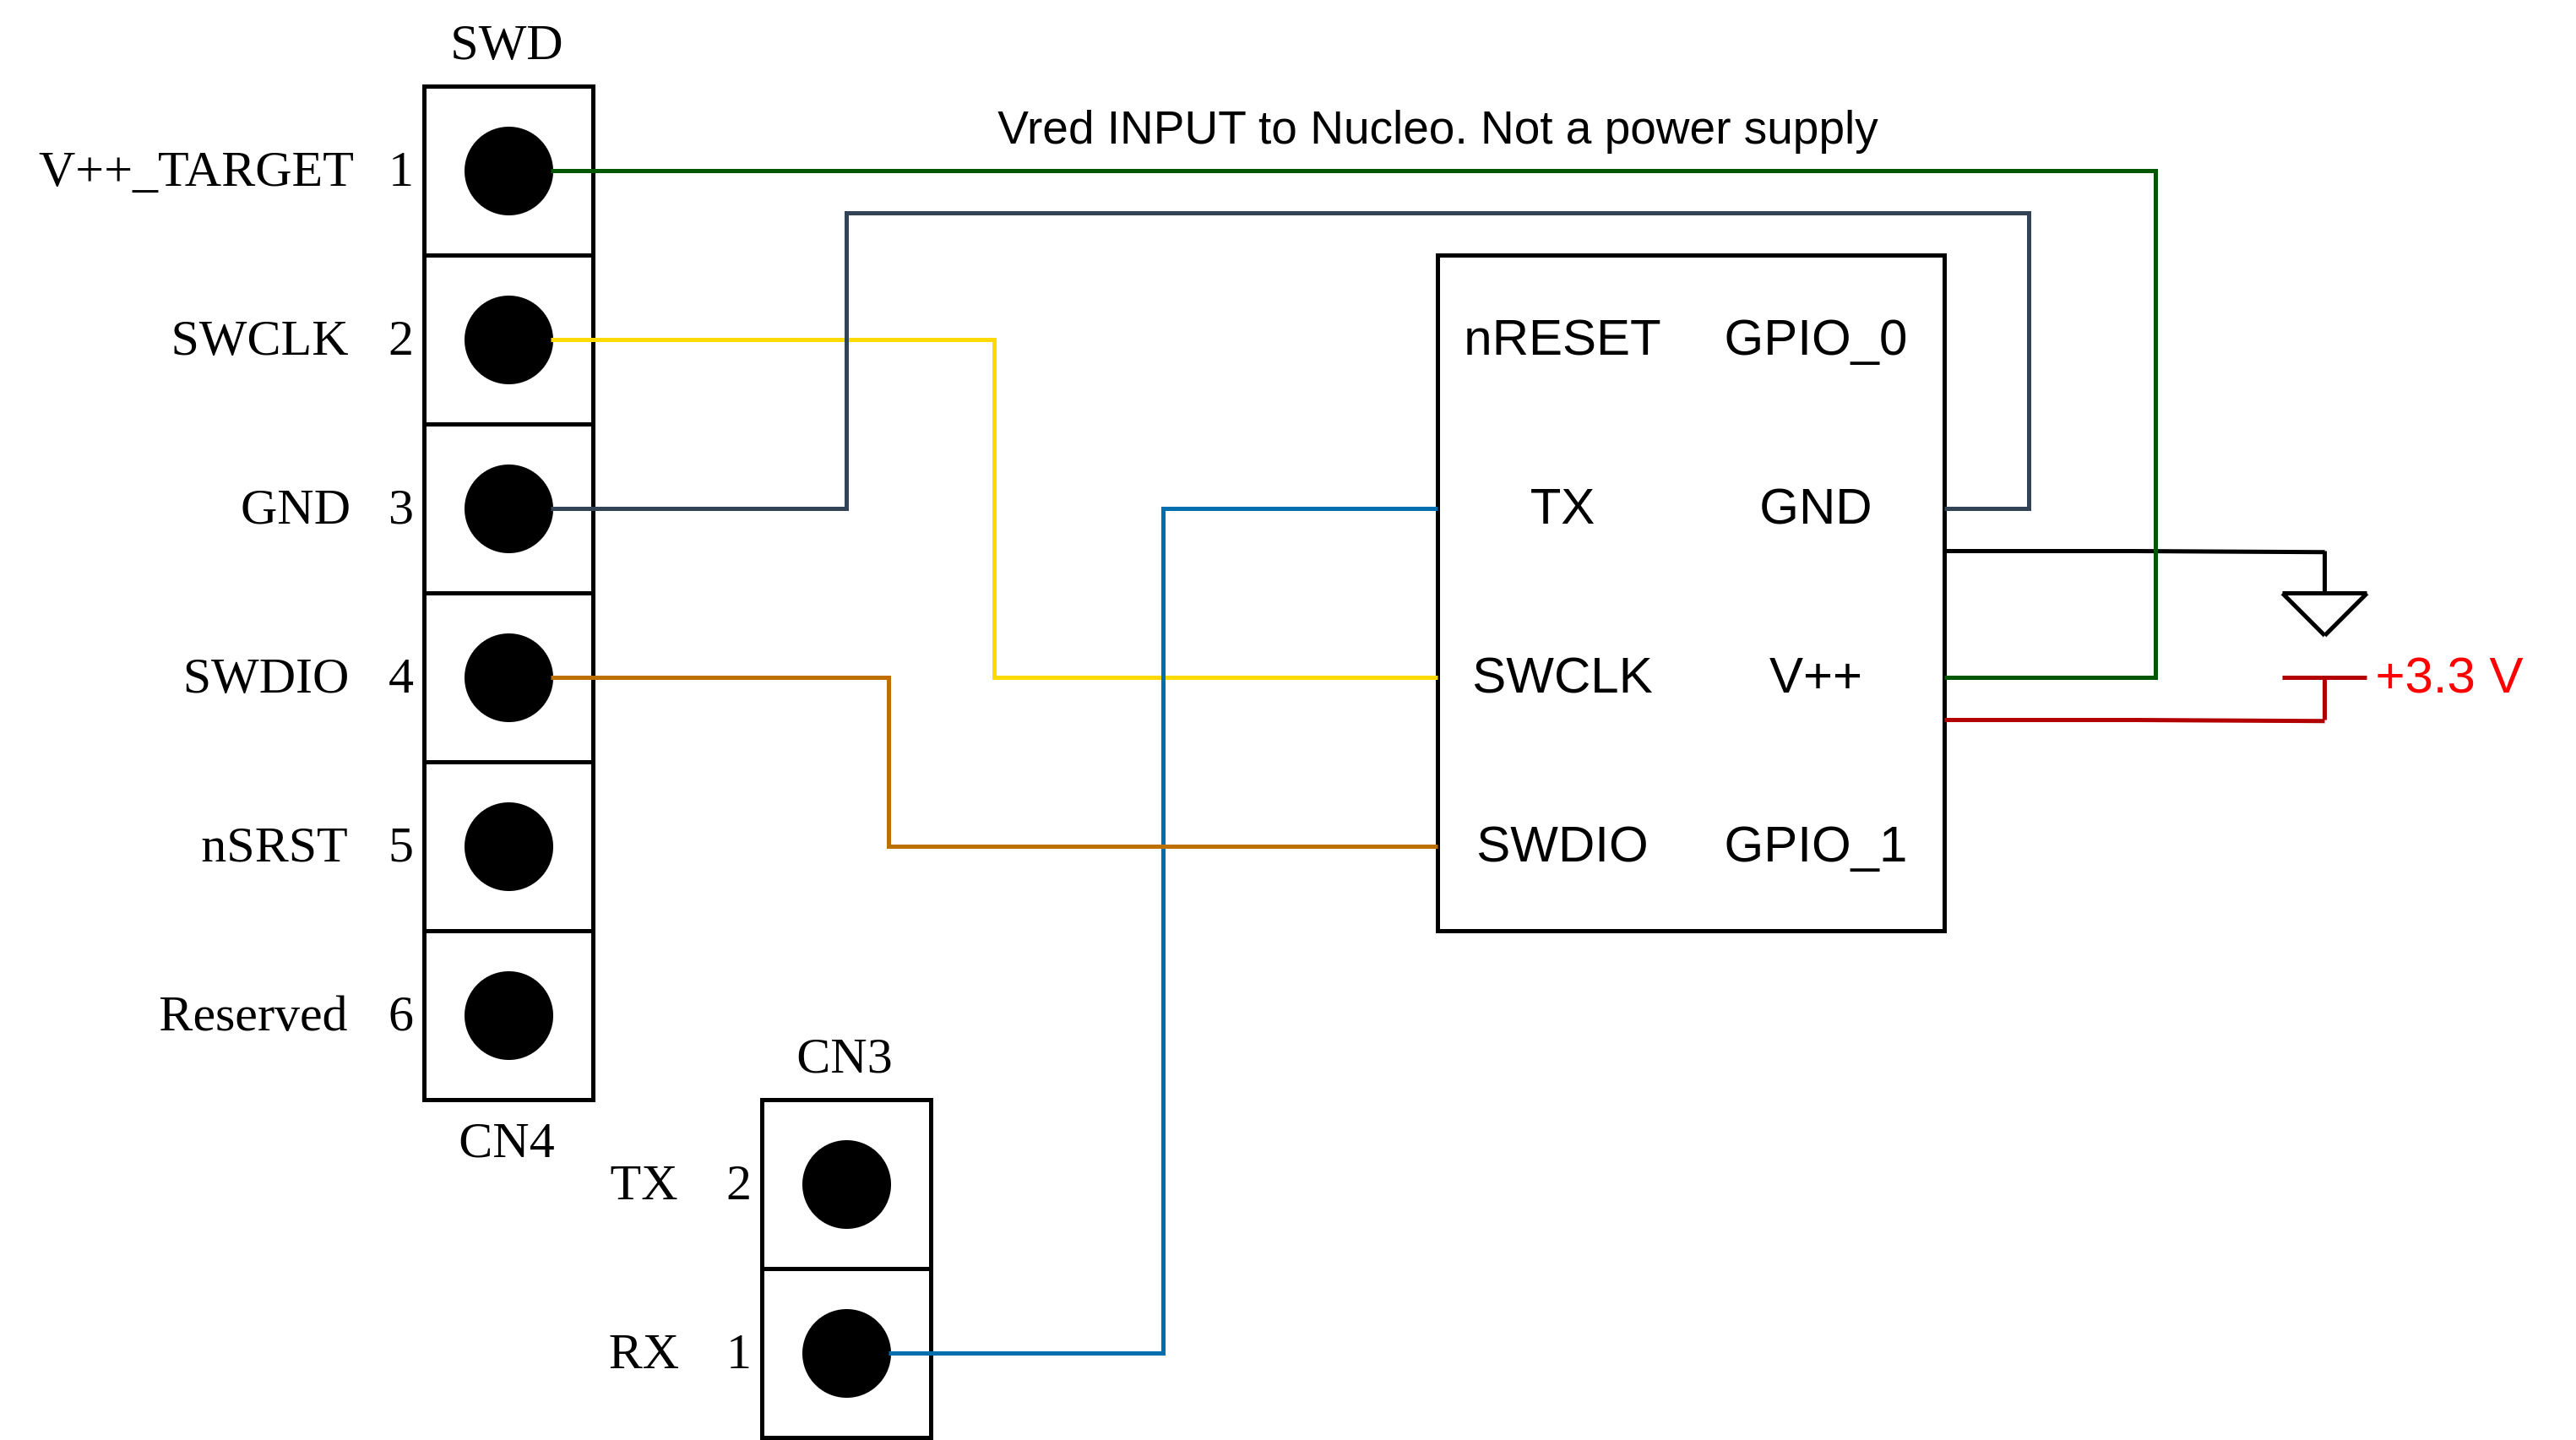
\includegraphics[width=0.8\textwidth]{figures/STLink_SWD_wiring.png}
  \caption{Diagram showing the connection between ST-LINK/V2-1 and a STM32 chip.}
  \label{fig:schematic_stlink}
\end{figure}

For communicating with the STM32-chip over \ac{USART} use the \textit{USART2} interface available on \textit{PA2} and \textit{PA3} of the STM32-chip. To enable the \ac{USART} communication between the ST-LINK/V2-1 and an external application, the related solder bridges \textit{SB13} and \textit{SB14} must be OFF (and \textit{SB62} and \textit{SB63} must be ON if using a Nucleo board and not having cut the board into an ST-LINK part and target STM32 part)\cite[p.~25]{STM32_Nucleo_user_manual}.

The ST-LINK/V2-1 is connected to the computer through \ac{USB}, and the STM32-chip is powered through the ST-LINK/V2-1. The STM32 is flashed with Visual Studio Code or the STM32CubeProgrammer\footnote{\url{https://www.st.com/en/development-tools/stm32cubeprog.html}}, which is a software tool to flash and debug STM32 microcontrollers. Here the STM32 can be debugged, which is done by setting breakpoints in the code and running the code step by step.

\begin{figure}[H]
    \centering
    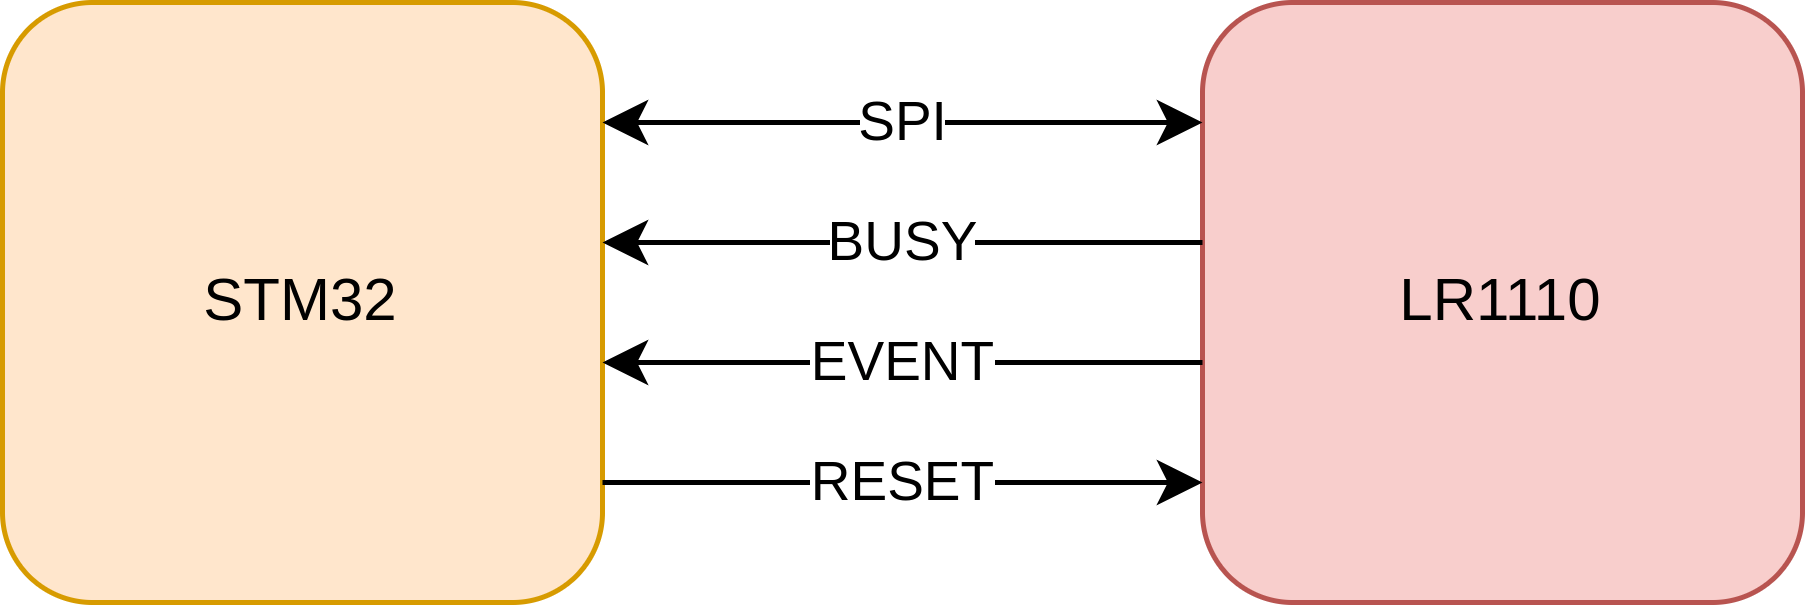
\includegraphics[width=0.7\textwidth]{figures/STM32_interface.png}
    \caption{Overview of the connection between STM32 and the host.}
\end{figure}

\subsection{Choosing transceiver firmware}
It would take up to 6 months longer to implement our own \ac{LoRa} stack

\subsection{Establishing communication with LR1110}
The STM32 and LR1110 communication is through \ac{SPI} (see fig.~\ref{fig:stm32_lr1110_interface}). The LR1110 exposes an \ac{API} which allows the STM32 to communicate with the LR1110 through a set of \ac{SPI} commands and responses.

\begin{figure}[H]
    \centering
    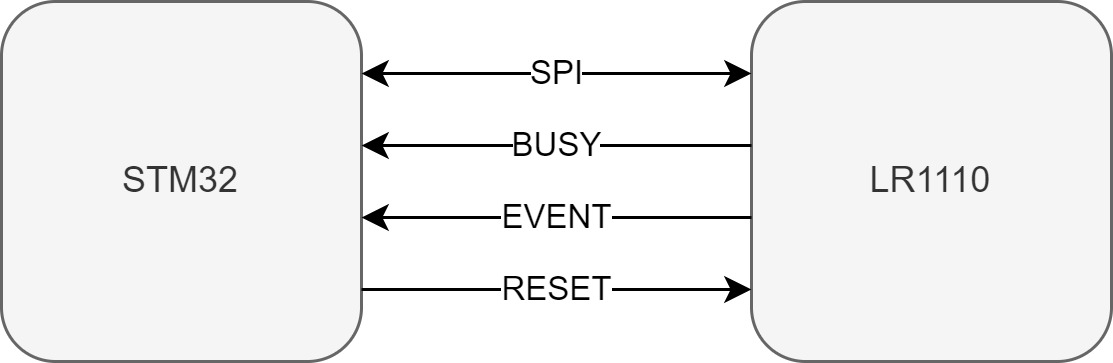
\includegraphics[width=0.6\textwidth]{figures/STM32_LR1110_interface.png}
    \caption{Interface between STM32 and LR1110.}
    \label{fig:stm32_lr1110_interface}
\end{figure}

The \textit{BUSY} signal is used as a handshake to indicate if the LR1110 is ready to accept a command. Therefore, it is necessary to check the status of \textit{BUSY} before sending a command.

The \textit{EVENT} signal is an output signal of the LR1110. This line signals to the STM32 that the device has an asynchronous event data pending. The event can be \ac{LoRaWAN} stack, \ac{GNSS}, or Wi-Fi events. The STM32 must use the \lstinline[style=C++]{GetEventSize(...)} command to determine the event size and \lstinline[style=C++]{GetEvent(...)} command to retrieve such data. The \textit{EVENT} signal stays high until all events are cleared. The STM32 must clear all the events before returning to sleep mode. This prevents the hit from missing the rising edge of the \textit{EVENT} signal when there is a new event. Secondly, this saves several \SI{}{\micro\ampere} of current consumption when the \textit{EVENT} signal is kept low by the LR1110.

Fig.~\ref{fig:event_example} shows an example of a Wi-Fi passive scan transaction. The STM32 sends a command to the LR1110 to scan for Wi-Fi \ac{AP}s. The LR1110 scans the Wi-Fi \ac{AP}s and stores the data in its internal memory. When the scan is complete, the LR1110 sets the \textit{EVENT} signal high to indicate that there is data to be read. The STM32 then reads the data from the LR1110 with \lstinline[style=C++]{GetEventsize(...)} and \lstinline[style=C++]{GetEvent(...)}, which afterwards then clears the \textit{EVENT} signal.

\begin{figure}[H]
    \centering
    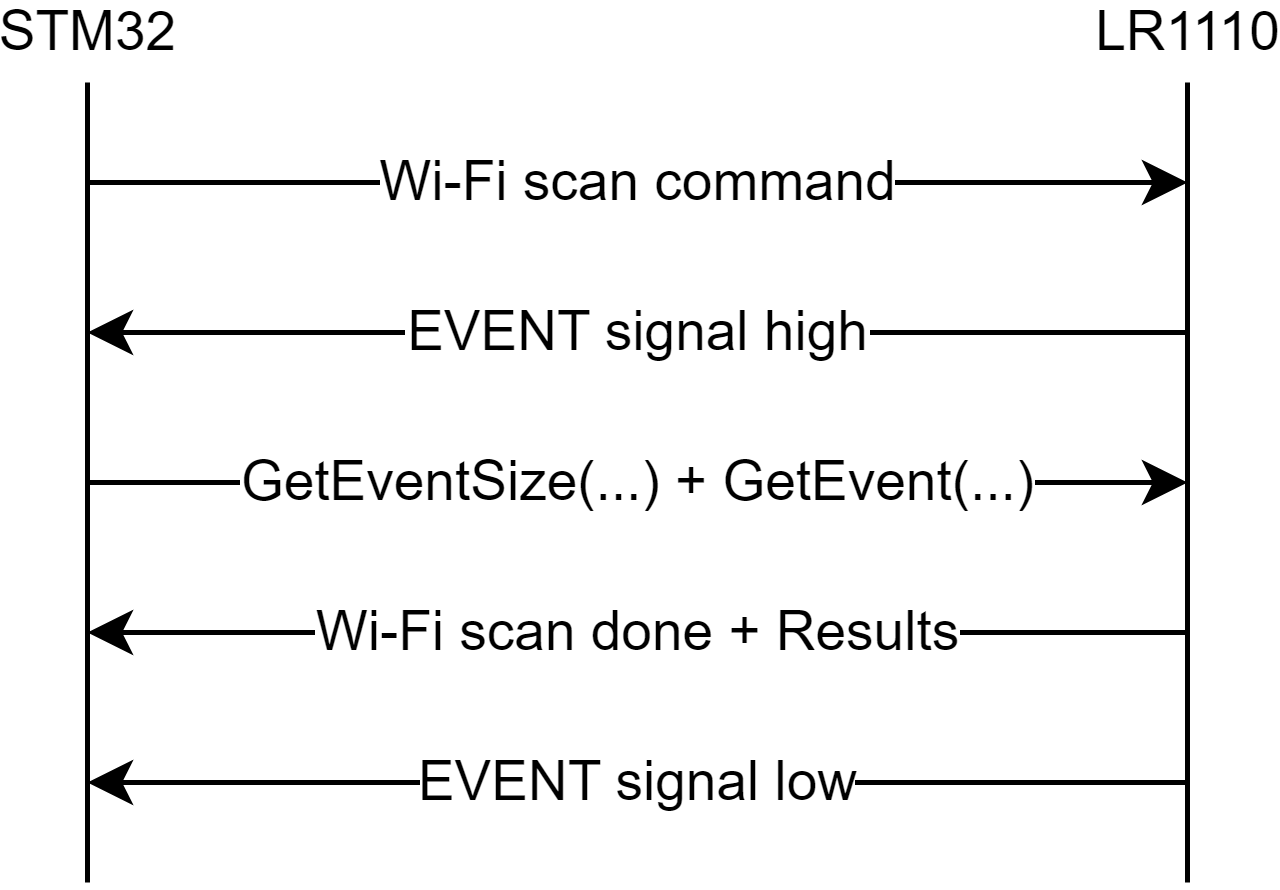
\includegraphics[width=0.5\textwidth]{figures/event_example.png}
    \caption{Example of Wi-Fi passive scan transaction. The transactions are read from top to bottom.}
    \label{fig:event_example}
\end{figure}

Some \ac{SPI} commands generate an immediate response by the LR1110 and therefore do not generate any \textit{EVENT} signal. Such as the command \lstinline[style=C++]{RequestTX(...)} as shown in fig.~\ref{fig:event_example_2}

\begin{figure}[H]
    \centering
    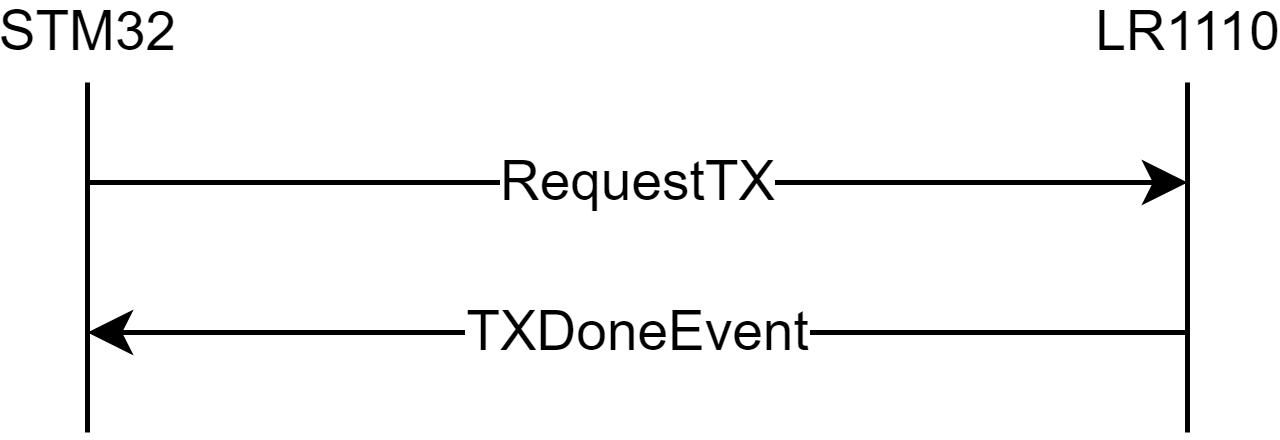
\includegraphics[width=0.5\textwidth]{figures/event_example_2.png}
    \caption{Example of a transaction which does not generate a \textit{EVENT} signal. The transactions are read from top to bottom.}
    \label{fig:event_example_2}
\end{figure}

\subsubsection{Write commands to LR1110}
When executing write commands (see fig.~\ref{fig:write_command}), the LR1110 transmits status registers and interrupt registers to the STM32 through the \textit{MOSI} pin, contingent upon the command opcode and its accompanying arguments. The host initiates by sending a 16-bit opcode (\textit{Op0} and \textit{Op1}), followed by the necessary arguments (\textit{Arg0}, \textit{Arg1}, etc.). Activation of the \textit{BUSY} signal occurs automatically upon the falling edge of the \textit{NSS}. Subsequently, once the LR1110 completes processing the command, the \textit{BUSY} signal is disengaged, signalling readiness to accept another command.

\iffalse
%wavedrom
{signal: [
  {name: 'BUSY', wave: '0.1.......................|0'},
  {name: 'NSS', wave: '10.......................1|.'},
  {name: 'MOSI', wave: 'x..5..5..7..7..7..7..7..xxxx', data: ['Op0', 'Op1', 'Arg0', 'Arg1', 'Arg2', 'Arg3', 'Arg4']},
  {name: 'MISO', wave: 'x..3..3..4..4..4..4..2..xxxx', data: ['Stat1', 'Stat2', 'IrqStat(31:24)', 'IrqStat(23:16)', 'IrqStat(15:8)', 'IrqStat(7:0)', '0']},
]}
\fi
\begin{figure}[H]
    \centering
    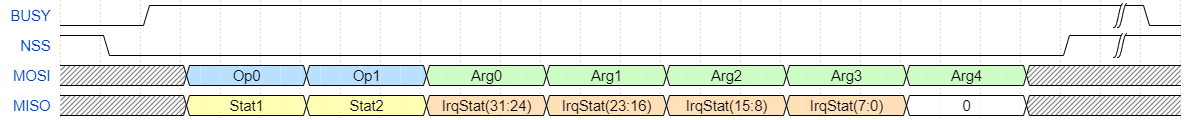
\includegraphics[width=1\textwidth]{figures/write_command.png}
    \caption{Write SPI command timing diagram.}
    \label{fig:write_command}
\end{figure}

\subsubsection{Read commands from LR1110}
Specific read commands extract LR1110 data, encompassing internal status or geolocation outcomes (fig.~\ref{fig:read_command} shows an example of reading data from the LR1110). The STM32 initiates by dispatching a 16-bit opcode (\textit{Op0} and \textit{Op1}), supplemented by arguments as necessary (\textit{Arg0}, \textit{Arg1}, etc.). Activation of the \textit{BUSY} signal occurs automatically upon the falling edge of the \textit{NSS}. Upon completion of data preparation by the LR1110, the \textit{BUSY} signal is disengaged. Subsequently, the host can retrieve the data by transmitting NOPs (\texttt{0x00} bytes) to sequentially extract the data via the \ac{SPI}.

\iffalse
%wavedrom
{signal: [
  {name: 'BUSY', wave: '0.1..............|0.1...........0'},
  {name: 'NSS', wave: '10..............1|.0...........1.'},
  {name: 'MOSI', wave: 'x..5..5..7..7..xxxxxx8..8..8..xxx', data: ['Op0', 'Op1', 'Arg0', 'Arg1', 'NOP', 'NOP', 'NOP']},
  {name: 'MISO', wave: 'x..3..3..4..4..xxxxxx3..6..6..xxx', data: ['Stat1', 'Stat2', 'IrqStat(31:24)', 'IrqStat(23:16)', 'Stat1', 'Rsp0', 'Rsp1']},
]}
\fi
\begin{figure}[H]
    \centering
    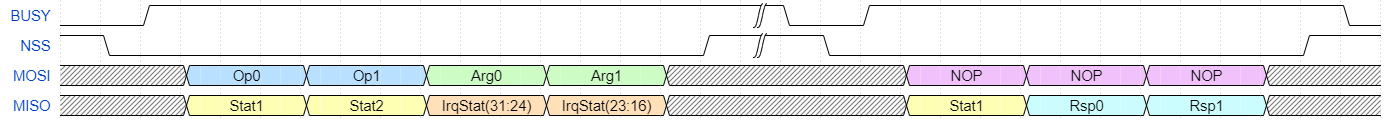
\includegraphics[width=1\textwidth]{figures/read_command.png}
    \caption{Read SPI command timing diagram.}
    \label{fig:read_command}
\end{figure}

One thing to notice is that when writing commands to LR1110 is that \textit{Stat1} and \textit{Stat2} refer to the former write command, not the current command that has just been sent. However, does \textit{Stat1} (from the read command) refer to the status for the current command.

\subsection{Implementation of tracking features}
In the following sections, we will describe how we implement geolocation. We will report on how we have implemented Wi-Fi scanning, satellite scanning, \ac{LoRa}-communication, and other notable features. We will also describe how we have implemented the power-saving features.

\subsubsection{Wi-Fi scanning}
Scanning of Wi-Fi \ac{AP}s is done by setting the channels and the time to scan each channel. The LR1110 will scan the Wi-Fi \ac{AP}'s and store the data in the internal memory. The STM32 chip can then read the data.

\subsubsection{Satellite scanning}
The LR1110 can scan for \ac{GPS}, BeiDou, and geostationary satellites. The scanning is done by setting the time to scan and then starting the scan. The STM32 chip can then read the data.

\subsection{Power minimising}
One of the other big sections in the report, as the title is ultra-low power. Here we will describe how we have tried to minimise power consumption.

What is ultra-low power and what is low power?

Maybe it won't be easy to write since it is probably an iterative process. We test which methods work best, and then change something until we have found the best method.


For a stable power supply, we are using the \ac{LDO} Voltage Regulators \hyperref[bom:xc6220]{XC6220B331MR} (datasheet: \sbref{app:hardware:XC6220}). The chip is a \SI{3.3}{\volt} voltage regulator with a input voltage ranging from \SI{1.6}{\volt} to \SI{6.0}{\volt} and a maximum output current of \SI{1000}{\milli\ampere}. The quiescent current is \SI{8}{\micro\ampere} and the dropout voltage is around \SI{20}{\milli\volt}. A voltage regulator is crucial for any battery-powered device. It has high power- and low power modes, which means the quiescent current and dropout voltage can be reduced if the device is in low power mode. When the output current is less than \SI{1}{\milli\ampere} (minimum), the quiescent current is reduced to \SI{8}{\micro\ampere}. If the output current becomes \SI{10}{\milli\ampere} (maximum) or more, the mode changes automatically to the high power mode and the chip returns to high-speed operation.

\subsection{PCB Design}
We are using EasyEDA\footnote{\url{https://easyeda.com/}} to design the \ac{PCB} and JLCPCB\footnote{\url{https://jlcpcb.com/}} to manufacture them.

\subsubsection{Impedance}
For determining the impedance and maintaining this throughout the \ac{PCB}, the layout of the components and stackup of the \ac{PCB} is important. We chose a 4-layer \ac{PCB} as this is preferable to optimise \ac{RF} \ac{PCB} layout, especially if there is dense routing. 

Any \ac{RF} line can potentially radiate or receive interfering signals, which is why the \ac{RF} trace between the antenna and the matching network is designed using a \ac{GCPW} structure as shown fig.~\ref{fig:gcpw}. This means that the second layer is one full layer for a clean ground plane below the \ac{RF} to minimize \ac{EMC} problems. The \ac{GCPW} is dimensioned to have a characteristic impedance equal to the antenna impedance, which we chose to be \SI{50}{\ohm}.

\begin{figure}[H]
    \centering
    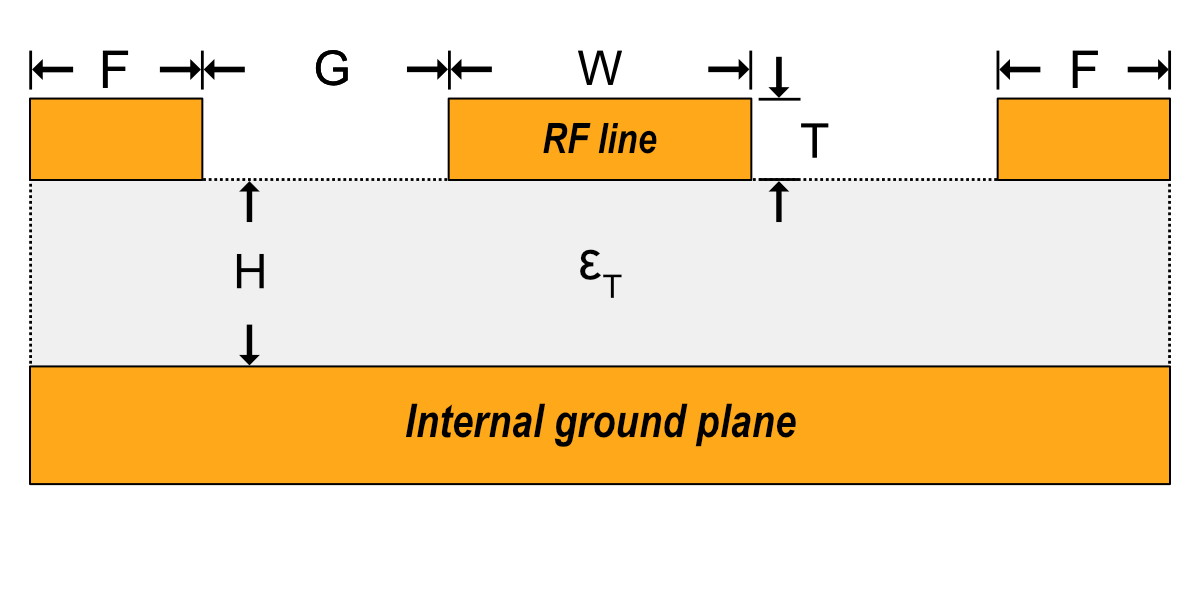
\includegraphics[width=0.6\textwidth]{figures/GCPW.png}
    \caption{Cross section of RF line layout. Here, the layer closest to the RF line is a ground layer, which will minimize any EMC issues.}
    \label{fig:gcpw}
\end{figure}

Choosing JCLPSB's JLC04101H-7628 Stackup has a dielectric constant of $\kappa = 4.4$ which will suit this project. The stackup is described in tab.~\ref{tab:pcb_stackup}.

\begin{table}[H]
    \centering
    \caption{Stackup of JLC04101H-7628 with PCB thickness of \SI{1.0}{\milli\meter}, outer copper weight of \SI{0.4}{\ounce}, and inner copper weight of \SI{0.5}{\ounce}\protect\footnotemark.}
    \label{tab:pcb_stackup}
    \begin{tabular}{lll}
    \textbf{Layer} & \textbf{Material Type} & \textbf{Thickness} \\ \hline
    Top Layer & \cellcolor{copper_green}Copper & \SI{0.035}{\milli\meter} \\
    Prepreg & 7628 & \SI{0.2104}{\milli\meter} \\
    Internal Ground Plane & \cellcolor{copper_green}Copper & \SI{0.0152}{\milli\meter} \\
    Core & \cellcolor{core_yellow}Core & \SI{0.45}{\milli\meter} \\
    Internal Power Plane & \cellcolor{copper_green}Copper & \SI{0.0152}{\milli\meter} \\
    Prepreg & 7628 & \SI{0.2104}{\milli\meter} \\
    Bottom Layer & \cellcolor{copper_green}Copper & \SI{0.035}{\milli\meter}
    \end{tabular}
\end{table}
\footnotetext{\url{https://jlcpcb.com/impedance}}

To calculate the transmission line characteristic impedance [$\Omega$] we will use Coplanar Waveguide by AppCAD \sbref{app:software:appcad}. Fig.~\ref{fig:appcad} shows the top layer, prepreg, and the internal ground plane.

\begin{figure}[H]
    \centering
    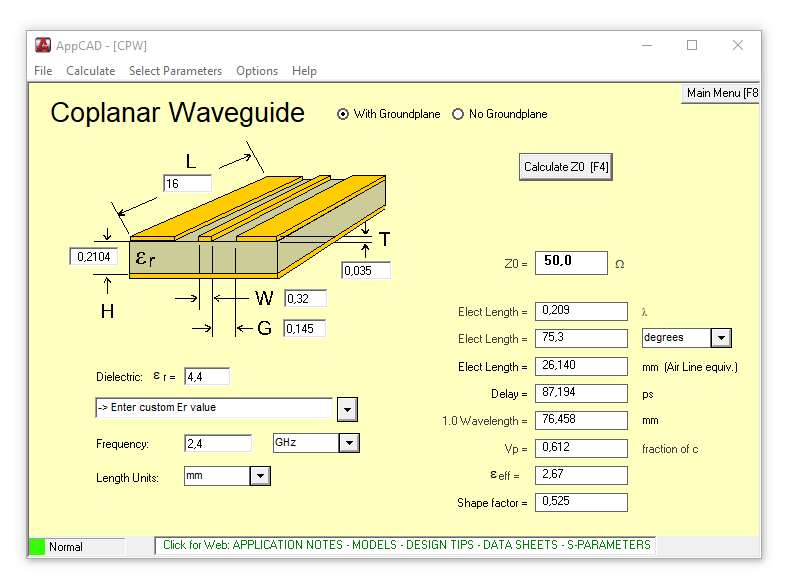
\includegraphics[width=1.0\textwidth]{figures/appcad_16.PNG}
    \caption{AppCAD Coplanar Waveguide: Calculating the impedance of the Wi-Fi RF line.}
    \label{fig:appcad}
\end{figure}

According to the PCB Design Guideline for LR1110, shall \textit{G}, \textit{W}, \textit{T}, \textit{H}, and $\epsilon_r$ (see diagram in fig.~\ref{fig:appcad}) be determined to ensure \SI{50}{\ohm} with coplanar waveguide with ground to \ac{RF} line. \textit{W} must be constant all along the \ac{RF} path, and if possible the same width as the components' pads. Furthermore, must the vias be stitches at a distance of a least $D = \lambda / 20 = \SI{52.915}{\milli\meter} / 20 = \SI{2.645}{\milli\meter}$ \cite[p.~9-11]{LR1110_pcb_design_guide}. The width of the ground on each side of the \ac{RF} line \textit{F} (see fig.~\ref{fig:gcpw}) must be larger than the width of the \ac{RF} line \textit{W} + the gap \textit{G}; $F > W + G$. Even if two \ac{RF} lines are close to each other (e.g. the \ac{RF} lines for \ac{LoRa}), then some ground should separate them to avoid coupling \cite[p.~20-21]{LR1110_pcb_design_guide}.

Most components on the \ac{RF} line have a width of around \SI{0.5}{\milli\meter}, which is why we chose \textit{W} to be \SI{0.5}{\milli\meter}. We chose the thickness of the \ac{PCB} to be \SI{1}{\milli\meter} and according to JLC04101H-7628 does \textit{T} have the height of \SI{0.035}{\milli\meter} and H would then be \SI{0.2104}{\milli\meter}. We would then choose \textit{G} to be \SI{0.5}{\milli\meter} so we are achieving an impedance of the RF line to be \SI{50}{\ohm}.

From this, we chose the \ac{PCB} design rules to be:
Track width: \SI{0.254}{\milli\meter} \\
Clearance: \SI{0.145}{\milli\meter} \\
Via diameter: \SI{0.25}{\milli\meter} \\
Via drill diameter: \SI{0.15}{\milli\meter}

\subsubsection{PCB design versions}
Our first version (fig.~\ref{fig:pcb_v1}) of the \ac{PCB} was designed to experiment with debugging and flashing the STM32-chip. It was a simple 2-layer \ac{PCB} with few components and oscillators for basic operations. We added \ac{LED}'s, \ac{USART} for debugging, and the footprint for the LR1110 chip, which we could test if we managed to flash and debug the STM32 chip. The LR1110 chip was added as a hat/shield to remove it better if something was not working immediately. After following instructions from sec.~\ref{sec:flash_debug_stm32} we quickly were able to flash the chip and later debug.

\begin{figure}[H]
    \centering
    \begin{minipage}[c]{0.49\textwidth}
        \centering
        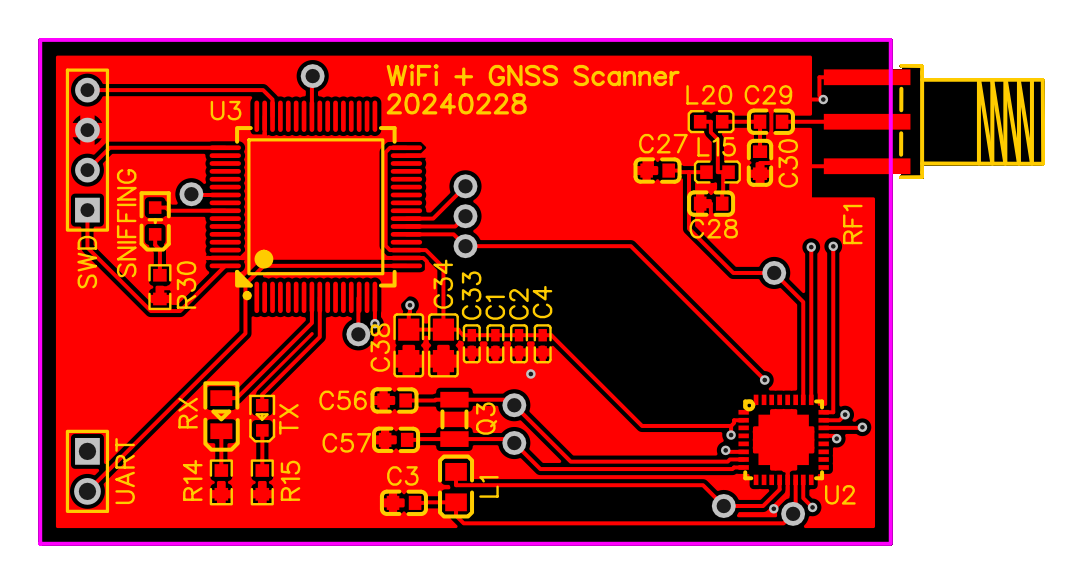
\includegraphics[width=\textwidth]{figures/PCB_v1.png}
    \end{minipage}
    \hfill
    \begin{minipage}[c]{0.49\textwidth}
        \centering
        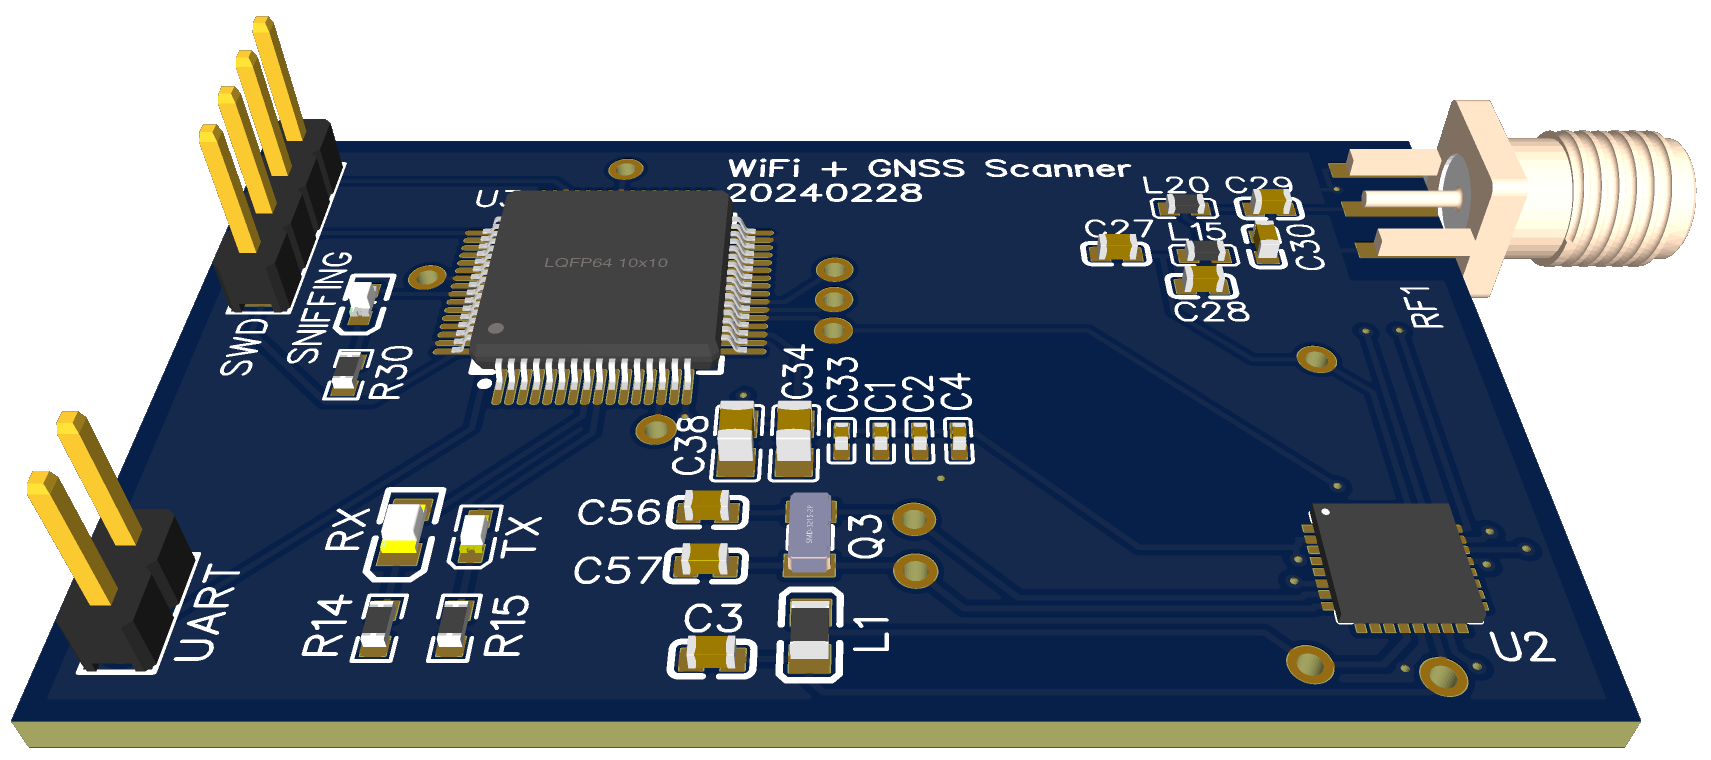
\includegraphics[width=\textwidth]{figures/PCB_v1_3D.png}
    \end{minipage}
    \caption{\nth{1} version of our PCB. \si{32} $\times$ \SI{54}{\milli\meter}.}
    \label{fig:pcb_v1}
\end{figure}

After the success of being able to fast flash and debug the system, we designed the second version (fig.~\ref{fig:pcb_v2}). This time, we designed a 4-layer \ac{PCB} for better routing and having a whole plane just for the ground. We added the \ac{RF}-lines for Wi-Fi, \ac{GNSS} and \ac{LoRa}. Furthermore, did we add a \SI{3.3}{\volt} voltage regulator, a reset switch, and the accelerometer to determine if the tracker has been moving.

\begin{figure}[H]
    \centering
    \begin{minipage}[c]{0.49\textwidth}
        \centering
        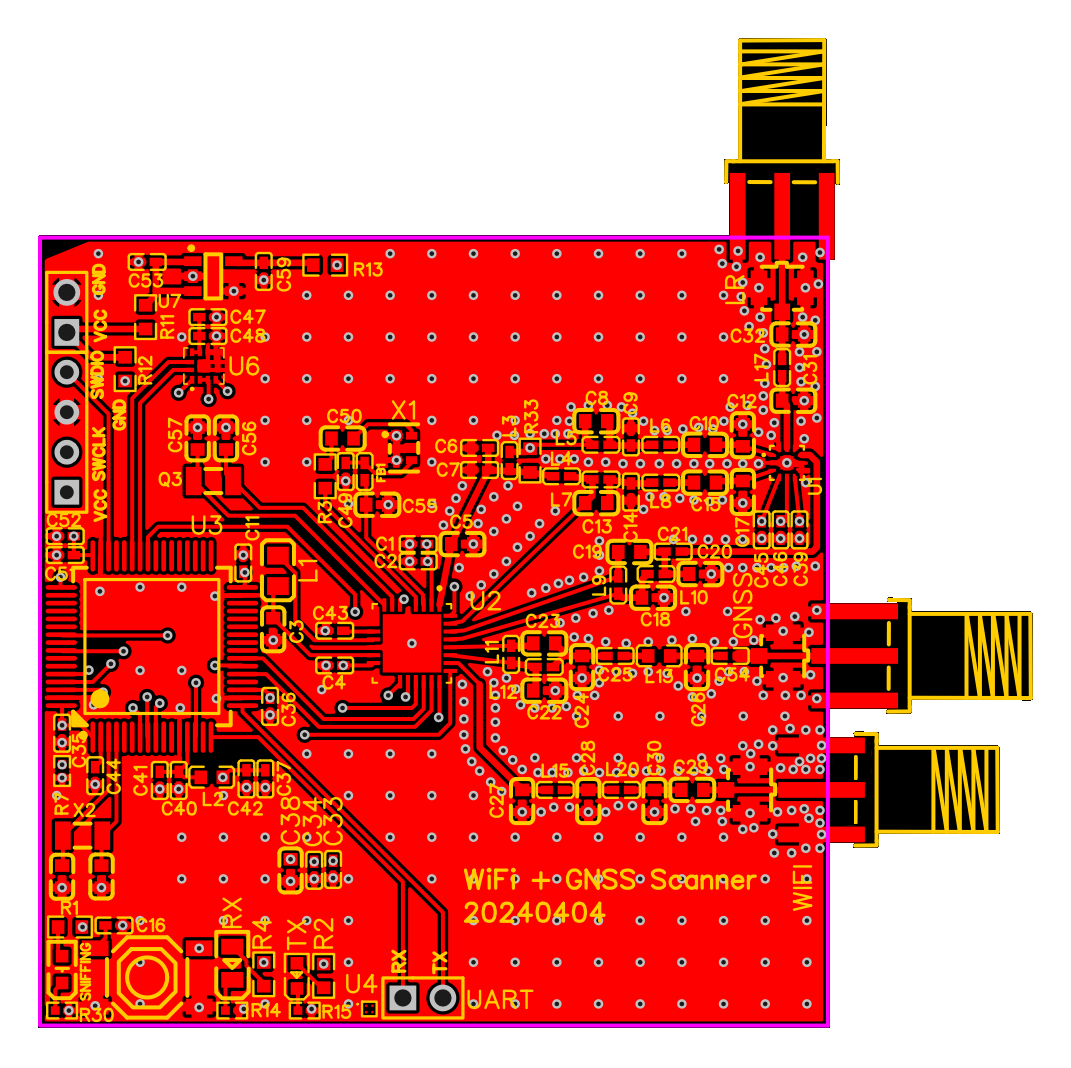
\includegraphics[width=\textwidth]{figures/PCB_v2.png}
    \end{minipage}
    \hfill
    \begin{minipage}[c]{0.49\textwidth}
        \centering
        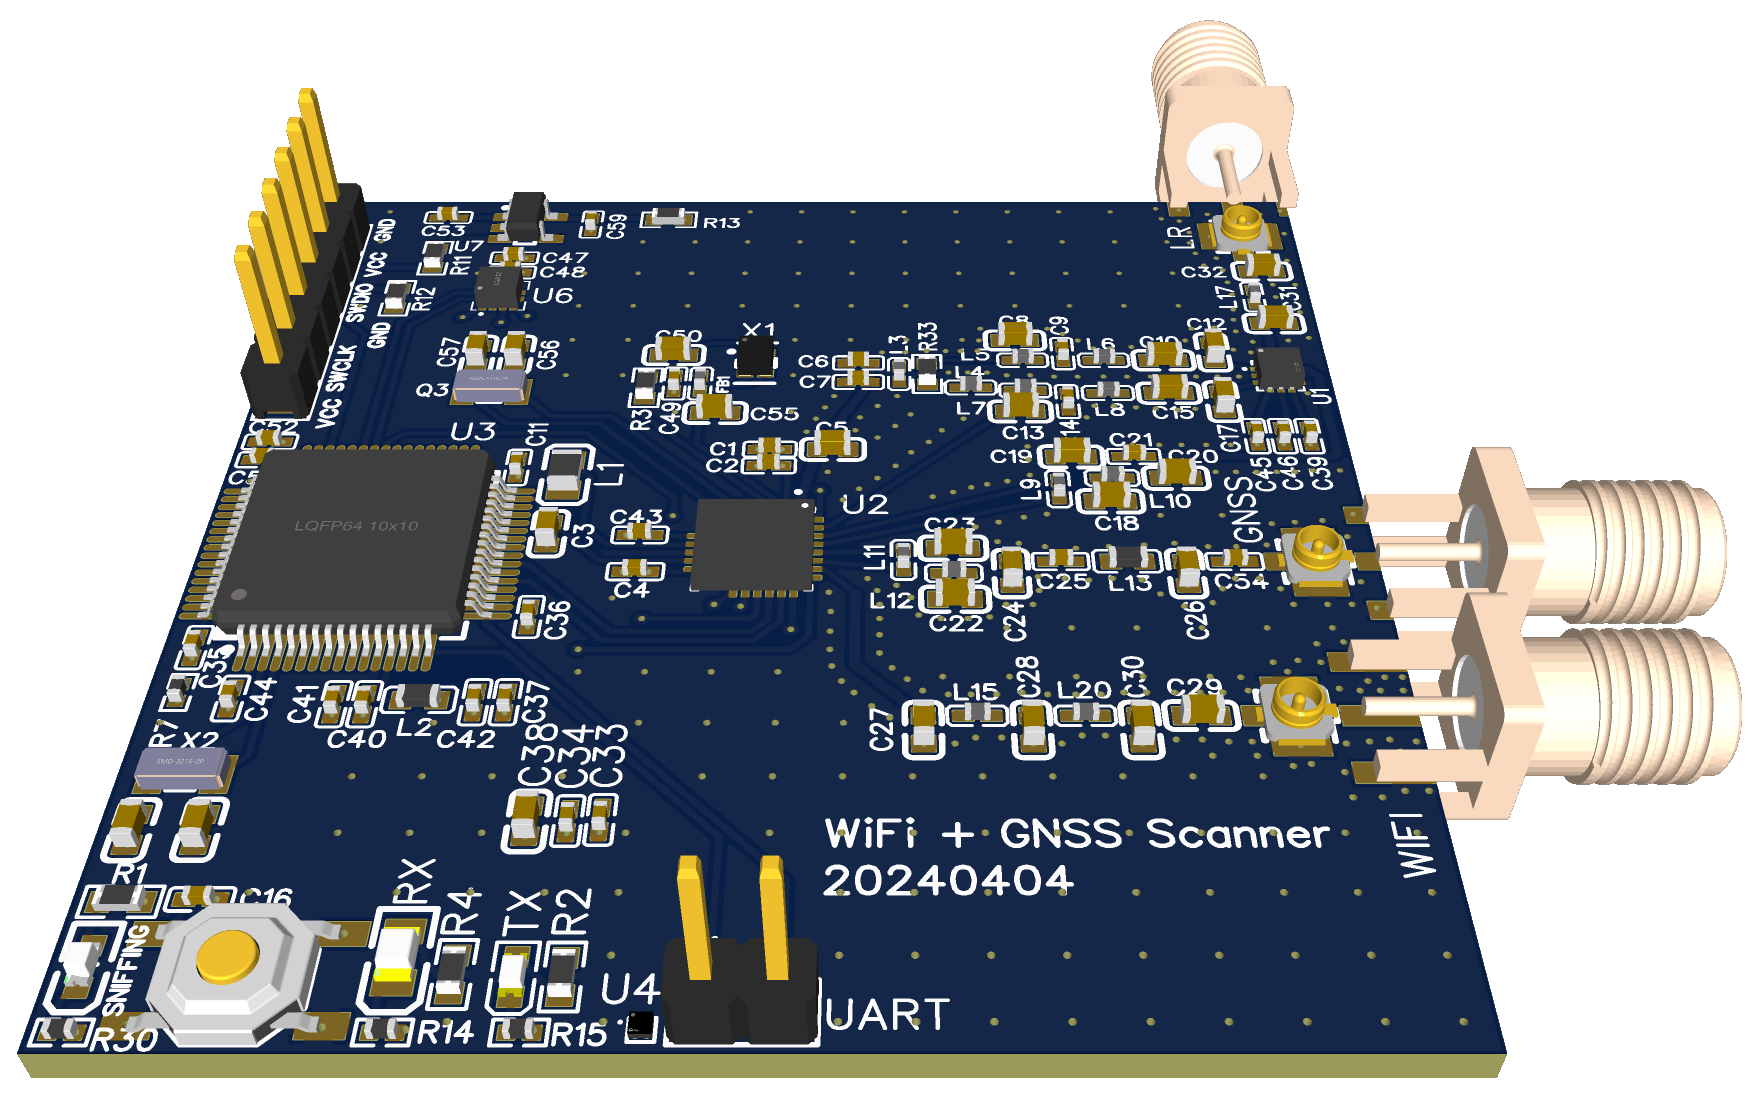
\includegraphics[width=\textwidth]{figures/PCB_v2_3D.png}
    \end{minipage}
    \caption{\nth{2} version of our PCB. \si{50} $\times$ \SI{50}{\milli\meter}.}
    \label{fig:pcb_v2}
\end{figure}

For the \nth{3} and final version of our \ac{PCB} (fig.~\ref{fig:pcb_v3}), we removed the \ac{LED}s and the reset button to make the board smaller (the pins were still there, which means that with the combination of a hat/shield still could be used). The size of the final \ac{PCB} is \si{33} $\times$ \SI{49}{\milli\meter}. We added the hall effect sensor and removed the big SMA antenna connectors instead of the smaller U.FL connectors.

\begin{figure}[H]
    \centering
    \begin{minipage}[c]{0.49\textwidth}
        \centering
        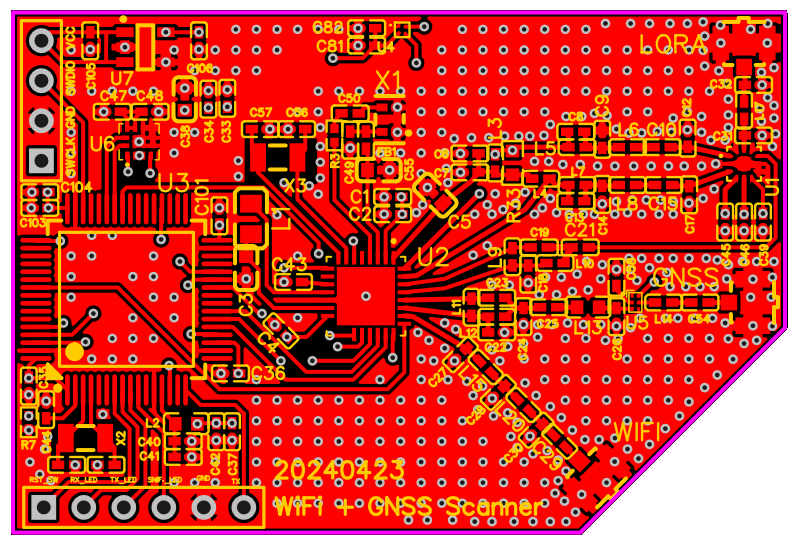
\includegraphics[width=\textwidth]{figures/PCB_v3.png}
    \end{minipage}
    \hfill
    \begin{minipage}[c]{0.49\textwidth}
        \centering
        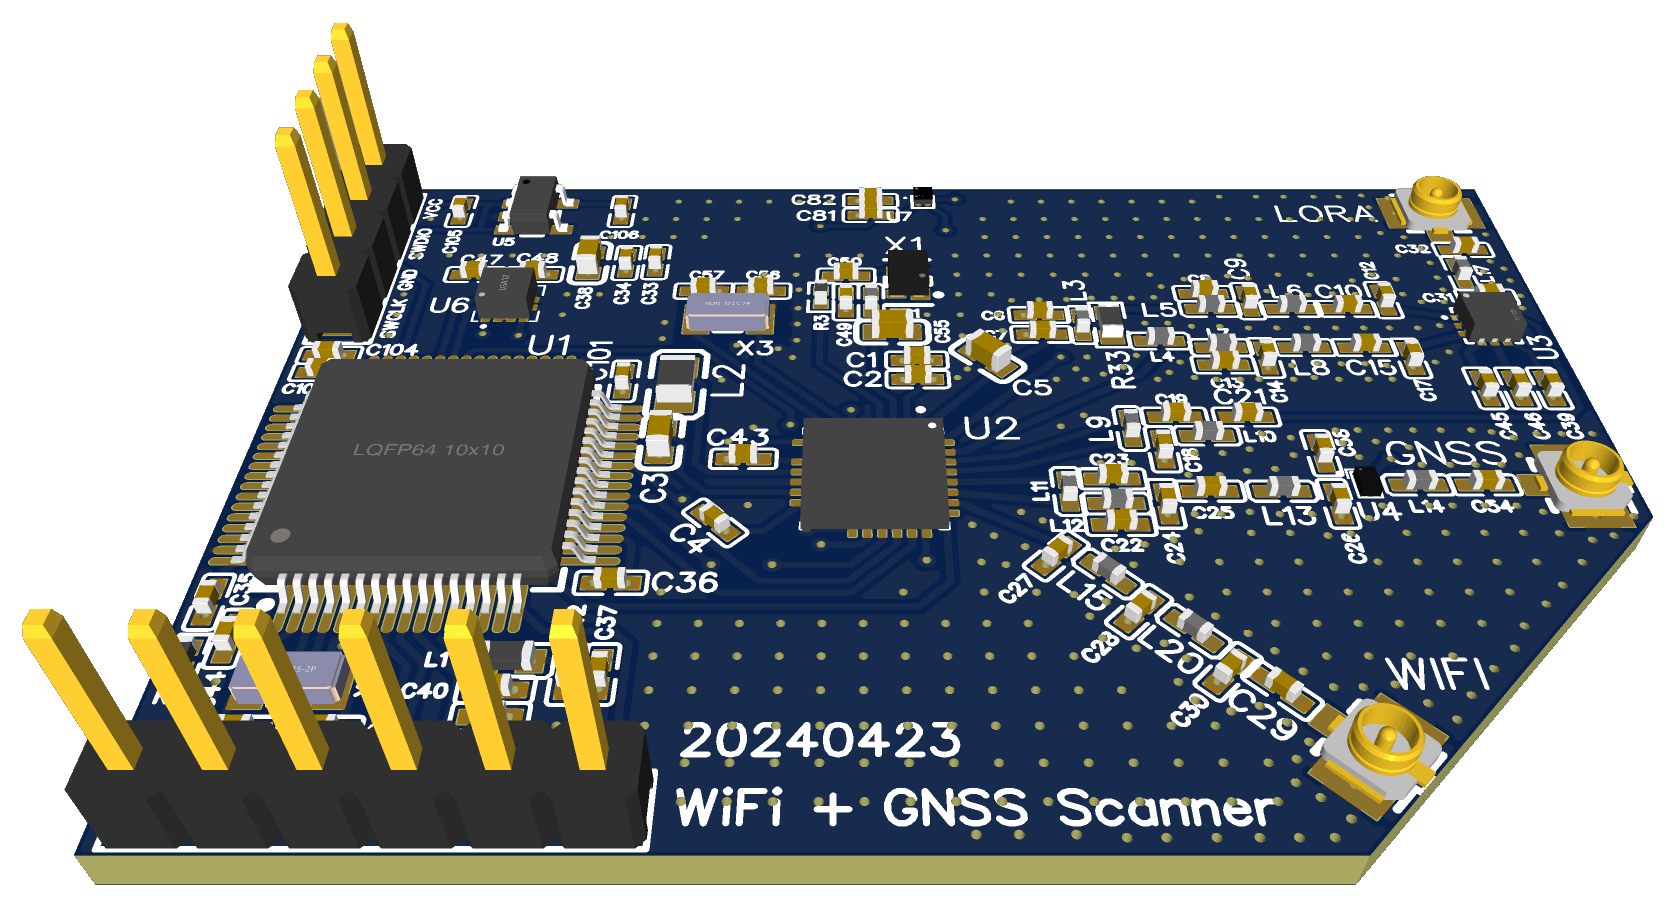
\includegraphics[width=\textwidth]{figures/PCB_v3_3D.png}
    \end{minipage}
    \caption{\nth{3} version of our PCB. \si{33} $\times$ \SI{49}{\milli\meter}. A larger version can be found in app.~\ref{app:PCB} and app.~\ref{app:3DView}}
    \label{fig:pcb_v3}
\end{figure}

As most of the components are tiny and sometimes will shorten when soldering on, X-ray images (see fig.~\ref{fig:x_ray}) need to be taken to verify no shorting of the components.

\begin{figure}[H]
    \centering
    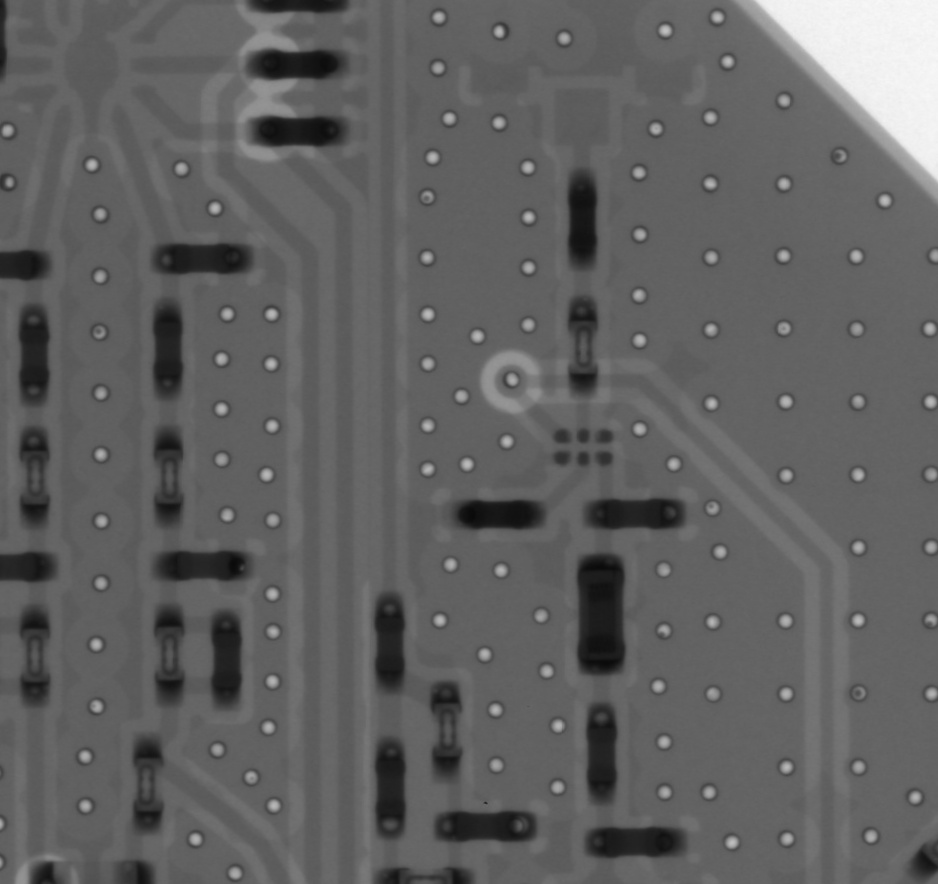
\includegraphics[width=0.5\textwidth]{figures/x_ray.jpg}
    \caption{X-ray (\SI{90}{\kilo\volt}, \SI{80}{\micro\volt}) image of the smallest components. The component (U4: \hyperref[bom:bga524n6e6327]{BGA524N6E6327}) with the 6 pins has a size of $1.1$ × \SI{0.7}{\milli\meter}.}
    \label{fig:x_ray}
\end{figure}

\subsubsection{Wiring diagram}
Fig.~\ref{fig:schematic} shows the wiring schematic of the tracker.

\begin{figure}[H]
    \centering
    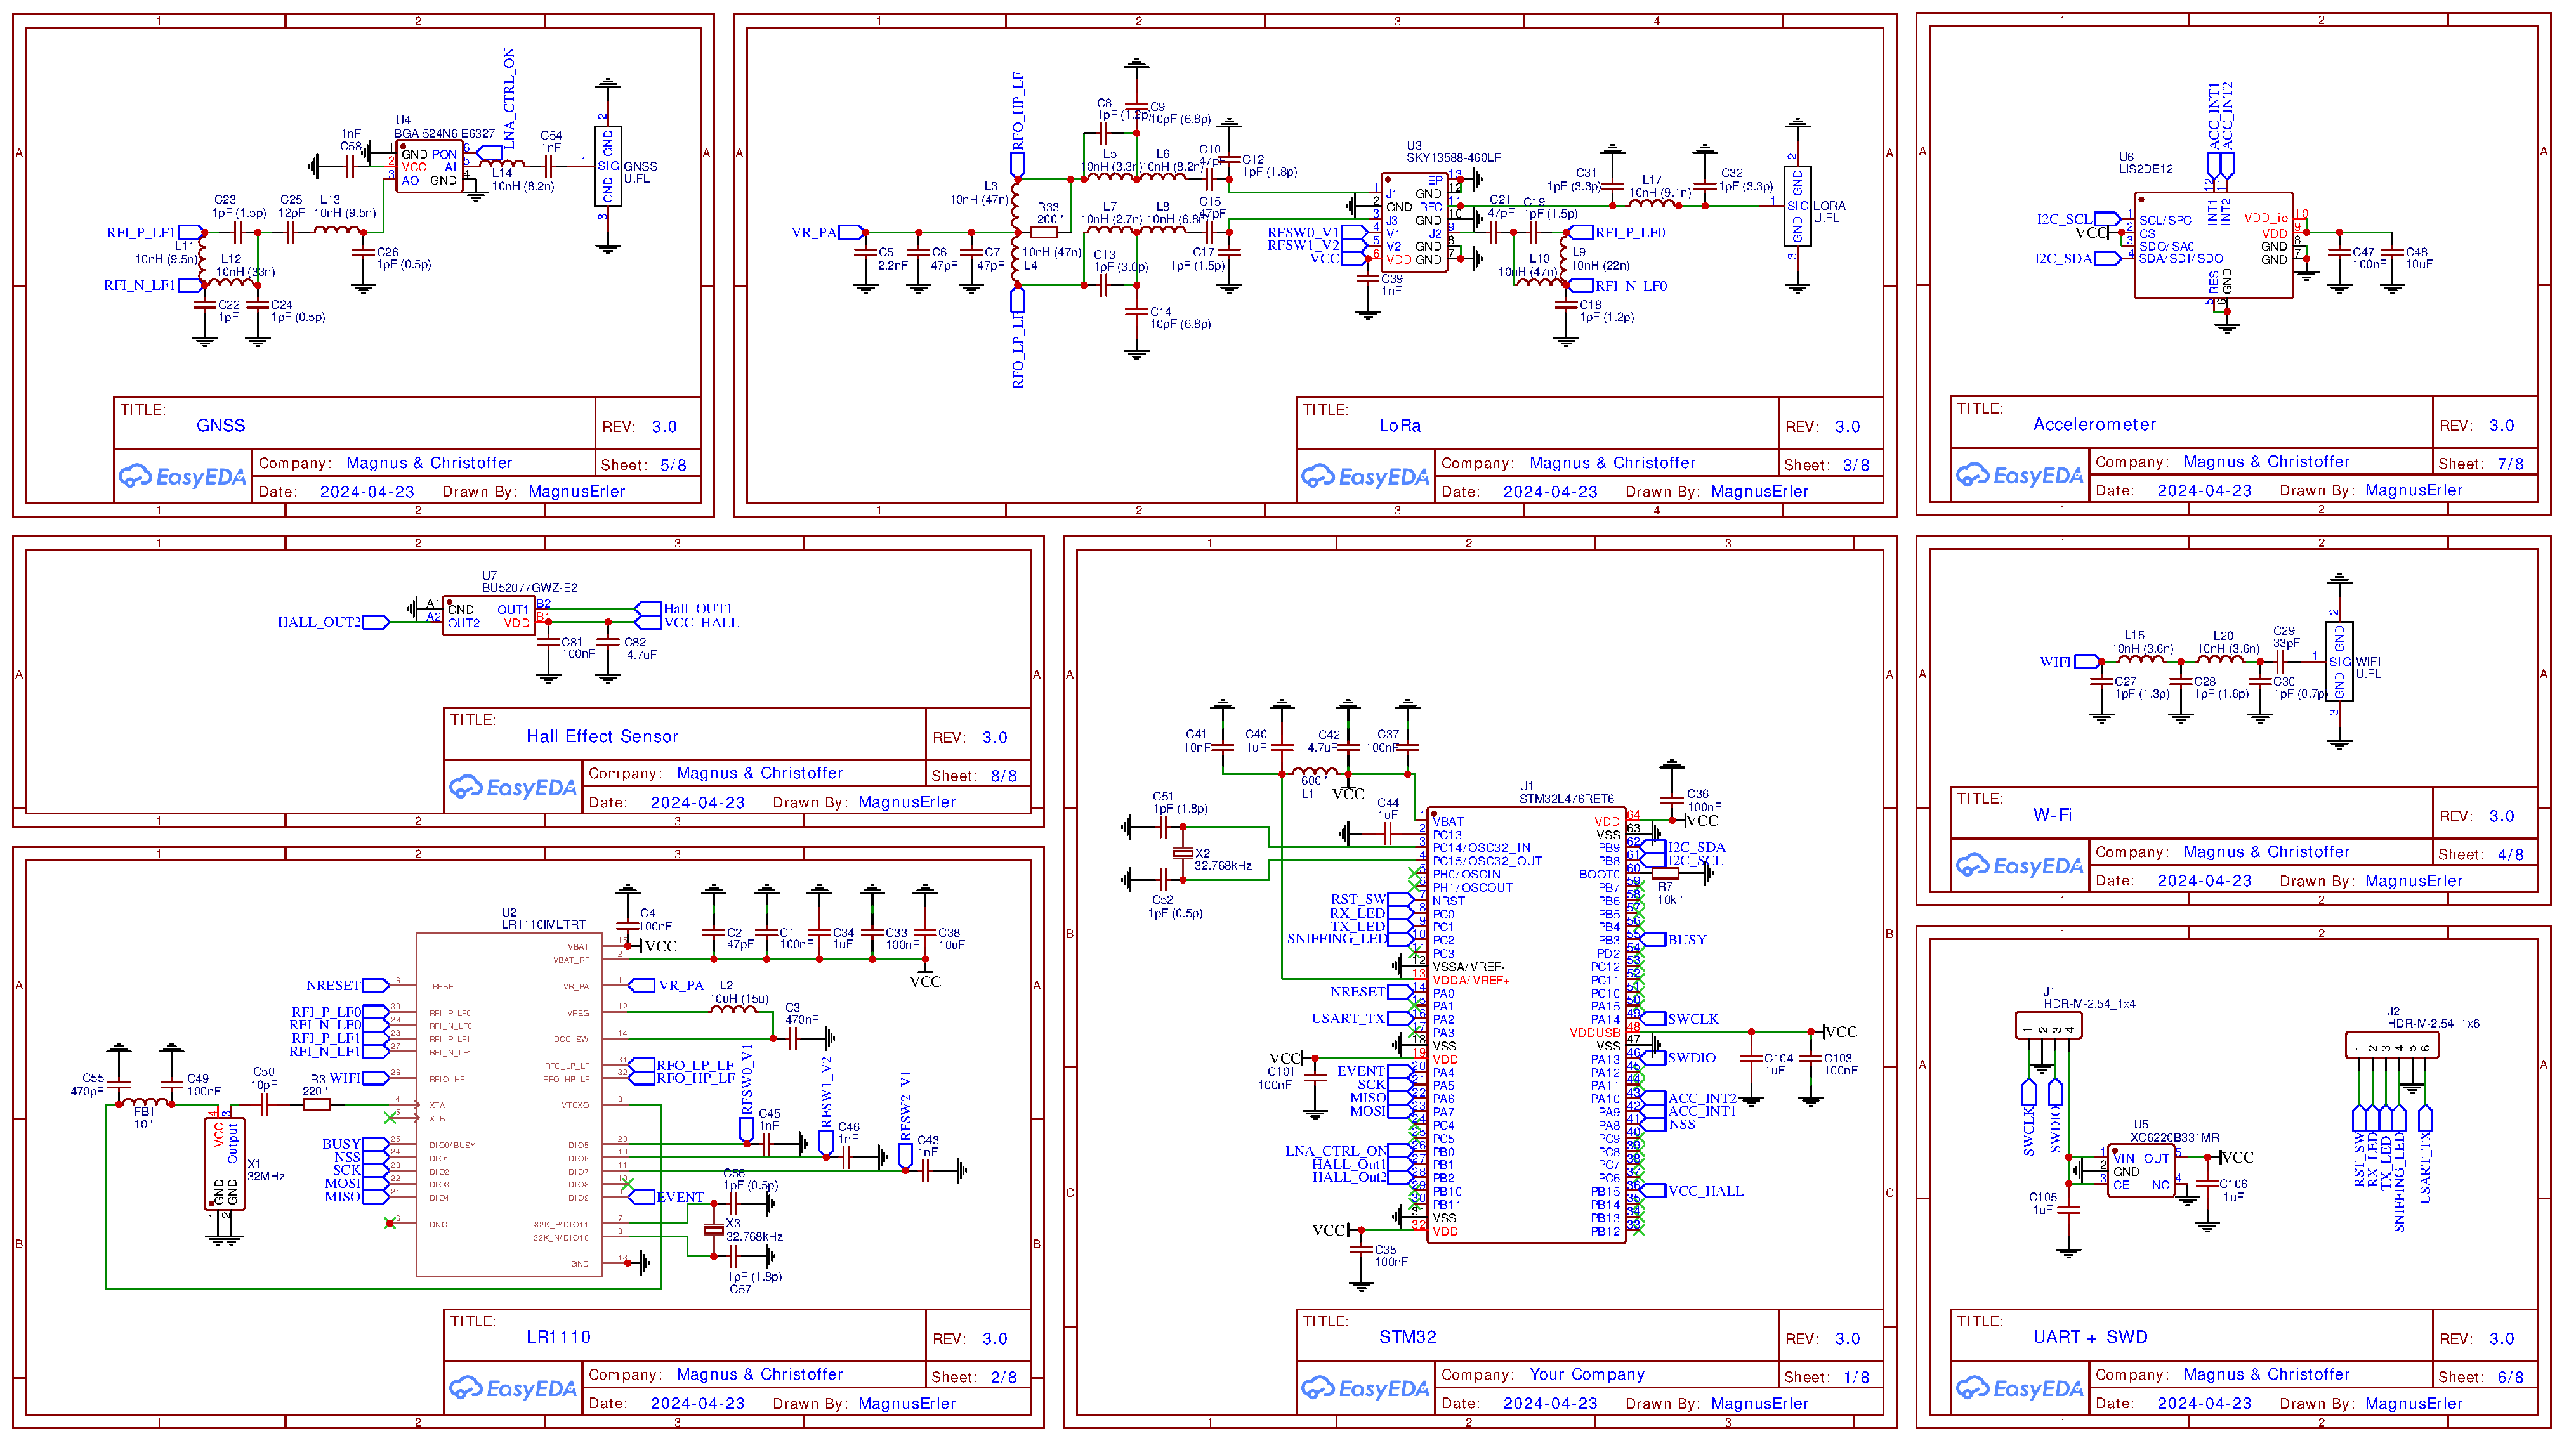
\includegraphics[width=1\textwidth]{figures/Schematic.pdf}
    \caption{Overview of the schematic. A larger schematic can be found in app.~\ref{app:wiringDiagram}.}
    \label{fig:schematic}
\end{figure}

\subsection{Case design}
We have set up requirements for this in the product requirements, so here you can say a little about how we prototype before the final design.
We have probably made several different prototypes. Chalk it up to the theory of prototypes.

\subsection{Cost}
LR1110 ordered from DigiKey Denmark\footnote{\url{https://www.digikey.dk/}} where it cost \SI{72.23}{\dkk} per chip. Ordering the rest from JLCPCB costs $\$2$ for the \ac{PCB} and an extra $\$35.61$ for the assembly of the components (5 \ac{PCB}). With shipping ($\$24.60$) and customs duties ($\$24.31$) the total amount is $\$86,52$. With the LR1110 chip, it is around \SI{193}{\dkk}.

The prices of key components are listed below in tab.~\ref{tab:BOM_keycomponents}. The rest of the \ac{BOM} in further detail can be viewed in app.~\ref{app:BOM}.

\begin{table}[H]
\centering
\small
\caption{BOM of key components.}
\label{tab:BOM_keycomponents}
\begin{tabular}{l|l|l|l|l|l}
Name & Designator & Footprint & Manufacturer Part & Manufacturer & Price [\$] \\ \hline
STM32L476 & U1 & LQFP-64 & STM32L476RET6 & ST & 2.924 \\
LR1110 & U2 & QFN-50 & LR1110IMLTRT & Semtech & 10.54 \\
SKY13588-460LF & U3 & QFN-12 & SKY13588-460LF & SKYWORKS & 2.254 \\
BGA524N6E6327 & U4 & TSNP-6 & BGA 524N6 E6327 & Infineon & 0.286 \\
XC6220B331MR & U5 & SOT23-5 & XC6220B331MR & TECH PUBLIC & 0.179 \\
LIS2DE12TR & U6 & LGA-12 & LIS2DE12TR & ST & 0.469 \\
BU52077GWZ & U7 & BGA-4 & BU52077GWZ & ROHM & 0.177 \\
\end{tabular}
\end{table}

\subsection{LoRaWAN communication}
Sending data from the Wi-Fi and \ac{GNSS} scans to the cloud is done through \ac{LoRaWAN}. The data is sent to the \ac{LoRaWAN} network server, which then forwards the data to the application server. The application server can then present the data in a user-friendly way. Sending the payload consumes a lot of power, so we have implemented power-saving features to only send the payload when the device has moved.

Suppose the accelerometer has not detected any movement in the period specified in the Wi-Fi or GNSS scan period. In that case, the device does not send the \ac{MAC} addresses of the Wi-Fi \ac{AP}s or \ac{GNSS} satellites. This would mean that the device has not moved and an additional scan for location is not necessary. Instead, it goes into sleep and checks again after either the Wi-Fi or \ac{GNSS} scan period has ended.

\subsubsection{Uplink communication}
If using Wi-Fi, each found\ac{MAC} address is appended and sent as one long payload on \ac{FPORT} 197. E.g. \texttt{00 2A 10 F4 A7 90 AA 8A FF 70 7E ED 6C 8B D3 CC F7 E0\textsubscript{(16)}} is a combination of \ac{MAC} address: \texttt{00 2A 10 F4 A7 90\textsubscript{(16)}}, \texttt{AA 8A FF 70 7E ED\textsubscript{(16)}}, and \texttt{6C 8B D3 CC F7 E0\textsubscript{(16)}}.

If using \ac{GNSS} the device sends XXX as a \ac{NAV} on \ac{FPORT} 198 or 192 depending on how many \ac{SV}'s the device can see

Setting it to \lstinline[style=C++]{SMTC_MODEM_SEND_MODE_STORE_AND_FORWARD} instead of normal \lstinline[style=C++]{SMTC_MODEM_SEND_MODE_UPLINK} will store the data in the LR1110 and send it when the device is in range of a \ac{LoRaWAN} gateway.

Tab.~\ref{tab:uplink_commands} shows the uplink commands that can be sent to the device.

\begin{table}[H]
\centering
\caption{Uplink commands.}
\label{tab:uplink_commands}
\begin{tabular}{l|l|l}
\ac{FPORT} & Usage & Payload \\ \hline
3 & Get temperature, battery voltage, and uptime & E.g. $26.4$ and $3.3$ \\
5 & Get firmware version & \\
6 & Get \ac{JoinEUI} & \\
7 & Get \ac{DevEUI} & \\
199 & LoRa Cloud requests (aka DM port or Stream port) & \\
201 & fragport & \\
\end{tabular}
\end{table}

The power consumption in sending 1 byte or 4 bytes over \ac{LoRaWAN} is not substantial


\subsubsection{Downlink communication}
Data from \ac{GNSS} can either be sent with \ac{GNSS} or \ac{GNSSNG}. \ac{GNSSNG} is used for multiple NAV messages.

Tab.~\ref{tab:downlink_commands} shows the downlink commands that can be sent to the device.

\begin{table}[H]
\centering
\caption{Downlink commands.}
\label{tab:downlink_commands}
\begin{tabular}{l|l|p{9cm}|l}
\ac{FPORT} & Payload & Usage & Default \\ \hline
1 & Scan period & \ac{GNSS} scan period [s] & \SI{120}{\second} \\
2 & Scan period & Set Wi-Fi scan period [s] & \SI{60}{\second} \\
192 & & \ac{GNSSNG}  & \\
197 & & Wi-Fi scan results to be forwarded to LoRa Cloud & \\
198 & & \ac{GNSS} port  & \\
199 & & LoRa Cloud requests ----- DM port ----- Stream port  & \\
201 & & fragport  & \\
\end{tabular}
\end{table}
% https://tektelic.com/wp-content/uploads/TEKTELIC_STORK_UG.pdf page 11
% https://www.chirpstack.io/docs/chirpstack/integrations/loracloud.html

Need to have:
Downlink
\ac{GNSS} scan interval
Wi-Fi scan interval

Uplink
Battery critical

Nice to have
Downlink
Temperature
Battery status

\subsection{Application}

ngrok\footnote{\url{https://ngrok.com/}}

One predominant requirement derived from our interviews was the need for a simple setup process for our device and an easy-to-use application for presenting the data.
Despite the growing adoption of \ac{LoRaWAN}-enabled devices, network setup remains considerably more intricate than devices that utilise Wi-Fi or cellular networks for data transmission which mostly work out of the box. Wi-Fi devices merely require access to an access point and a network password, and cellular devices only necessitate a SIM card, where the technical part of joining the network is left to the network provider. \ac{LoRaWAN}-enabled device on the other hand entails several additional considerations. You need to think about provisioning, choice of network and network coverage, network protocol version and regional requirements.

Let us look at how one would add an LR1110 end device to the network and start getting geolocation pings
\begin{enumerate}
    \item Get device info from the chip (\ac{DevEUI}, PIN and \ac{JoinEUI})
    \item Create a user on Loracloud.com 
    \item Create an application on Loracloud.com
    \item Choose the \ac{LoRaWAN} network provider or implement your own gateway
    \item Change bindings for Loracloud.com application to allow join requests from chosen \ac{LoRaWAN} network provider
    \item Claim device on Loracloud.com Join Server
    \item Claim device on Loracloud.com Modem \& Geolocation Services
    \item Create user at chosen \ac{LoRaWAN} network provider
    \item Create application at chosen \ac{LoRaWAN} network provider
    \item Register device at chosen \ac{LoRaWAN} network provider with correct frequency plan, \ac{LoRaWAN} version, regional parameters, \ac{JoinEUI} and \ac{DevEUI}
    \item Create API token on Loracloud.com Modem \& Geolocation Services
    \item Setup integration between \ac{LoRaWAN} network provider application and Loracloud.com Modem \& Geolocation Services.
\end{enumerate}

Looking at the above list, one can see that setting up an LR1110 device is a technical ?

We therefore chose to make our application setup less technical and provide a more coherent and easy-to-use user experience.

Setup for our application:
1. Read \ac{DevEUI}, PIN on the package.
2. 
3.
4.
5.
6.
7.
8.

If a new location has been found but it is close to the previous location (e.g. radius of \SI{5}{\meter}) that location will not be shown on the map, but however updated as the device has been seen.

Future work:
Låst til TheThingsNetwork
Låst til EU
Stadig lidt teknisk. Man skal finde application keys og certificate

When developing a web application, there is no need to reinvent the wheel and code everything from scratch. One could use technologies such as vanilla HTML, CSS and JavaScript, however using a front-end framework or library as a scaffold for building your application, offers enhanced efficiency, consistency and scalability. Frameworks provide a standardised structure with easier maintainability and features like cross-browser compatibility, strong community support, and built-in security.

\subsubsection{Client-side}
Many different frameworks or libraries could have been chosen for the client side of our application. We chose React as we have prior experience with it and its prominence as one of the most used web technologies (source: \url{https://survey.stackoverflow.co/2023/#technology-most-popular-technologies}), offered extensive availability of libraries, online resources and community support.
Leaflet\footnote{\url{https://leafletjs.com/}} was chosen for displaying the map, as it is the leading open-source JavaScript library for mobile-friendly interactive maps. We could have chosen to use Google's map service, as it would have offered familiarity (a wish we saw in our interviews). However this service isn't free, and will therefore add a cost to the product, and the price was the bigger factor for all users, and the interaction with Leaflet is quite similar to how you interact with Google Maps.

\subsubsection{Server-side}
Express
SQLite3